%%%%%%%%%%%%%%%%%%%%%%%%%%%%%%%%%%
%%% TODO:
%%% Po pierwsze opisac interfejsy szeregowe ogolnie, czym sa etc..
%%% Kodowanie w USB3.0  dokladniej opisac, zastosowania, rysunki, przebiegi, czas, power
%%% Jakos te tytuly napisac czytelniej, konsekwencja w mala/duza litera (pamietalem o tym kiedys)
%%% Wstep do kazdego rozdzialu + podsumowanie
%%% Dluzszy wstep, rozwinac poczatkowa wfaze (1.5 str), motywacja pracy
%%% opisy rozdzialow zbic w jeden akapit
%%% Proces weryfikacji biblioteki
%%% Podsumowane do poprawy
%%% Platforma testowa
%%% Odstepy do poprawy
%%% Testy -  - przyklad w mgr Łukasz Jachymczyk ~2012
%%% rysunki wektorowe
%%% range fix
%%% Sierotki + wdowy do poprawy
%%% 
%%% podzielenie wynikow (teoretyczne, praktyczne, porownanie, podsumowanie)
%%% dopisac dodatki (zewnetrzne biblioteki, zawartosc CD etc..)
%%%
%%%
%%%
%%%
%%%
%%%
%%%
\documentclass{BscUS}
\usepackage{setspace}
\usepackage{graphicx}
\usepackage{polski}
\usepackage{subfig}
\usepackage[utf8]{inputenc}
%\usepackage[OT4]{fontenc}
\usepackage{verbatim}
%\usepackage{libertine}
\usepackage{fourier}
\usepackage[T1]{fontenc}
\usepackage{enumitem}
\setitemize{noitemsep,topsep=0pt,parsep=0pt,partopsep=0pt}
\usepackage{float}
\usepackage{amsmath}
\usepackage{gensymb}
\usepackage{physics}
\usepackage{siunitx}
\usepackage{nameref}
\usepackage{listings}
\usepackage{indentfirst}

\usepackage{color}

\usepackage{array}

 \usepackage{multirow}
 \usepackage[table,xcdraw]{xcolor}

\usepackage{fancyvrb}
\DefineVerbatimEnvironment{packet}{Verbatim}{xleftmargin=40mm,baselinestretch=1,samepage=true}
\DefineVerbatimEnvironment{code}{Verbatim}{xleftmargin=36pt,samepage=true,tabsize=4}

\usepackage{fancyhdr}
\pagestyle{fancy}

\fancyhf{}
\fancyhead[RE,LO]{\leftmark}
\fancyhead[LE,RO]{\thepage}
\renewcommand{\headrulewidth}{1pt} 

%%\renewcommand{\labelenumi}{\Roman{enumi}}

\graphicspath{{img}}

\title{Opracowanie systemu szybkiego przesyłania danych z wykorzystaniem standardu USB}

\author{Łukasz Pawlik}
\promoter{dr inż. Bartosz Mindur}
\where{Kraków}
\when{2015}


\definecolor{mygreen}{rgb}{0,0.6,0}
\definecolor{mygray}{rgb}{0.5,0.5,0.5}
\definecolor{mymauve}{rgb}{0.58,0,0.82}

\lstset{ %
  backgroundcolor=\color{white},   % choose the background color; you must add \usepackage{color} or \usepackage{xcolor}
  basicstyle=\footnotesize,        % the size of the fonts that are used for the code
  breakatwhitespace=false,         % sets if automatic breaks should only happen at whitespace
  breaklines=true,                 % sets automatic line breaking
  captionpos=b,                    % sets the caption-position to bottom
  commentstyle=\color{mygreen},    % comment style
  deletekeywords={...},            % if you want to delete keywords from the given language
  escapeinside={\%*}{*)},          % if you want to add LaTeX within your code
  extendedchars=true,              % lets you use non-ASCII characters; for 8-bits encodings only, does not work with UTF-8
  frame=single,	                   % adds a frame around the code
  keepspaces=true,                 % keeps spaces in text, useful for keeping indentation of code (possibly needs columns=flexible)
  keywordstyle=\color{blue},       % keyword style
  language=C,                 % the language of the code
  otherkeywords={*,...},            % if you want to add more keywords to the set
  numbers=none,                    % where to put the line-numbers; possible values are (none, left, right)
  numbersep=5pt,                   % how far the line-numbers are from the code
  numberstyle=\tiny\color{mygray}, % the style that is used for the line-numbers
  rulecolor=\color{black},         % if not set, the frame-color may be changed on line-breaks within not-black text (e.g. comments (green here))
  showspaces=false,                % show spaces everywhere adding particular underscores; it overrides 'showstringspaces'
  showstringspaces=false,          % underline spaces within strings only
  showtabs=false,                  % show tabs within strings adding particular underscores
  stepnumber=2,                    % the step between two line-numbers. If it's 1, each line will be numbered
  stringstyle=\color{mymauve},     % string literal style
  tabsize=2,	                   % sets default tabsize to 2 spaces
  title=\lstname                   % show the filename of files included with \lstinputlisting; also try caption instead of title
}



\begin{document}

\pagestyle{plain}

% ******* title and statement page *******
\maketitle

\makestatement

\newpage
\thispagestyle{plain}
Merytoryczna ocena pracy przez Opiekuna:
\vspace{\stretch{14}}


Ocena końcowa pracy przez Opiekuna: 
\vspace{\stretch{1}}

\hspace{2cm} Data: \hspace{6cm}  Podpis: ..............................
\vspace{\stretch{1}}
\pagebreak
\newpage
\thispagestyle{plain}
Merytoryczna ocena pracy przez Recenzenta:
\vspace{\stretch{14}}


Ocena końcowa pracy przez Recenzenta: 
\vspace{\stretch{1}}

\hspace{2cm} Data: \hspace{6cm}  Podpis: ..............................
\vspace{\stretch{1}}
\pagebreak
\newpage
\thispagestyle{plain}
\vspace*{\stretch{18}}


% ************* contents list ************
\clearpage
%\pagenumbering{arabic}
\tableofcontents

\newpage


\addtocontents{toc}{\protect\setcounter{tocdepth}{1}}
\chapter{Wstęp}
\label{beginChapter}
\pagestyle{fancy}
W dobie dzisiejszych możliwości rosną również wymagania i oczekiwania. Dotyczy to prawie każdego aspektu dzisiejszej egzystencji począwszy od spraw osobistych poprzez finansowe aż po możliwości uzyskiwania danych. Rozwój technologi, zwłaszcza w zakresie elektroniki, w przeciągu minionego ćwierćwiecza stał się imponujący. Udało się doprowadzić różne skomplikowane układy scalone do rozmiarów wielkości pudełka zapałek, których złożoność obliczeniowa przekracza najśmielsze oczekiwania z przed kilku lat. Dla współczesnego człowieka problemem okazuje się czas, zawsze jest go za mało w praktycznie każdej sferze życia. Jest on również istotny w rozwoju technologi oraz uzyskiwaniu konkretnych danych pomiarowych.
\newline
\indent Dzisiejsze urządzenia pomiarowe laboratoryjne jak i medyczne (oraz inne) mają za zadanie zbieranie i przesyłanie danych celem późniejszej wizualizacji lub analizy za pomocą dedykowanego oprogramowania. Dane te z reguły są wysyłane w określonym formacie dla danego urządzenia a co za tym idzie rozmiar wysyłanych danych musi być większy niż w wypadku danych wysyłanych bajt po bajcie.
\newline
\indent Człowiek odkąd powstał pierwszy komputer rozpoczął walkę z problemem komunikacji między urządzeniami. Zostało opracowanych wiele standardów komunikacji, niektóre projekty zostały skazane na zapomnienie, inne odniosły sukces i zdominowały urządzenia. Takim standardem jest z pewnością USB, czyli Uniwersalna Magistrala Szeregowa (dokładny opis wraz z rysem historycznym w rozdziale \ref{USBStandardChapter}). Na dzień dzisiejszy większość urządzenia dla których konieczna jest komunikacja z komputerem osobistym (wyłączając sieci Ethernetowe \footnote{Ethernet - standard sieci lokalnych} oraz WiFi\footnote{WiFi - technologia sieci bezprzewodowych}) posiada interfejs USB.
\newline
\indent Celem niniejszej pracy było opracowanie szybkiego przesyłania danych używając standardu USB. Przez szybkie rozumiana jest tutaj prędkość nie mniejsza niż 140Mbit/s (17,5 MB/s) \footnote{1 B = 8 bit}.
\newline
\indent Pierwszym zadaniem, które musiało zostać wykonane przed rozpoczęciem realizacji implementacji oprogramowanie było wybranie hardwaru, które miało pełnić role urządzenia testowego (nie jest możliwe wykonanie testów przesyłu danych po interfejsie USB bez urządzenia odbierającego dane). Dokładny opis wybranego urządzenie został umieszczony w rozdziale \ref{microcontrollerChapter}. Kolejnym zadaniem był odpowiedni wybór biblioteki spełniającej założenia projektu. Istnieje wiele implementacji bibliotek udostępniających API \footnote{API (ang. Application Programming Interface) - zestaw funkcji oraz innych narzędzi umożliwiających wykorzystanie możliwości danej biblioteki} dla interfejsu USB. W rozdziale \ref{librariesChapter} szczegółowo zostały opisane dwie najczęściej używane z których pierwsza używana jest zarówno pod systemem Windows jak i pod systemem Unix natomiast użycie drugiej z nich możliwe jest tylko pod systemami Windows. Dodatkowo zostało przedstawione krótkie uzasadnienie wyboru.
\newline
\indent Kolejnym etapem podczas projektowania oprogramowania było dokładne zaplanowanie jak przebiegać będą testy. Istotnym elementem było to iż wykonanie ich bez urządzenia zewnętrznego było niemożliwe. Wtedy też należało opracować wejściowy jak i zwracany format danych dla każdego testu. Po opracowaniu podstawowych wymagań i testowych restrykcji dla aplikacji możliwe było przystąpienie do pisania aplikacji. Opis aplikacji wraz z implementacją znajduje się w rozdziale \ref{implementationChapter}.
\newline
\indent Ostatnim i zarazem najważniejszym elementem pracy jest zestawienie otrzymanych wyników wraz z oczekiwaniami. Całość została opisana w rozdziale \ref{resultsChapter} i zawiera konkretne wnioski na temat realizacji projektu oraz ogólnych możliwości interfejsu USB. W rozdziale zawarte jest dodatkowo zestawienie i interpretacja otrzymanych wyników w zakresie synchronicznego oraz asynchronicznego przesyłania danych za pomocą USB. Została w nim zaprezentowana dodatkowa symulacja, aby sprawdzić zachowanie interfejsu w mniej dostępnym środowisku.


\iffalse
%%old introduction
Rozwój technologi, zwłaszcza w zakresie elektroniki, w przeciągu minionego ćwierćwiecza stał się imponujący. Udało się doprowadzić różne skomplikowane układy scalone do rozmiarów wielkości pudełka zapałek, których złożoność obliczeniowa przekracza najśmielsze oczekiwania z przed kilku lat. 

Celem niniejszej pracy było uzyskanie możliwie największej prędkości przesyłu danych pomiędzy urządzeniem zewnętrznym a komputerem osobistym w obu kierunkach, z wykorzystaniem wspomnianego interfejsu. 

W pracy przedstawiono najważniejsze fakty historyczne dotyczące standardu USB (zawarte w rozdziale \ref{USBStandardChapter}, a także scharakteryzowano zachowania interfejsu w dwóch istotnych trybach: synchronicznym oraz asynchronicznym. Kolejne rozdziały zawierają opis standardu USB, rozpatrywanego w kontekście sprzętowym i oprogramowania.

Rozdział \ref{librariesChapter} posłużył do opisu zastosowanych bibliotek USB, do których między innymi należą: libUSB oraz winUSB. Obie z nich służą do komunikacji z urządzeniami z portami USB. Pierwsza używana jest zarówno pod systemem Windows jak i pod systemem Unix natomiast użycie drugiej z nich możliwe jest tylko pod systemami Windows.

W kolejnym rozdziale znajduje się charakterystyka poszczególnych funkcji biblioteki libUSB użytej w projekcie. Rozdział \ref{libUsbChapter} opisuje szczegółowo warunki użycia danej funkcji, wraz z zwracanym wartościami. 

Rozdział \ref{microcontrollerChapter} stanowi krótki opis mikrokontrolera użytego w projekcie. Zawiera on również rysunek poglądowy opisujący poszczególne elementy mikrokontrolera w tym ważne z punktu widzenia projektu.

Rozdział \ref{implementationChapter} zawiera szczegóły implementacyjne. Opisuje klasę bazową wraz z podstawowymi ustawieniami oraz ustawienia i sposób wykonania testu dla poszczególnych interfejsów.

Podsumowanie przeprowadzonych symulacji zawarte zostało w rozdziale \ref{resultsChapter}. Zawiera on zestawienie i interpretację otrzymanych wyników w zakresie synchronicznego oraz asynchronicznego przesyłania danych za pomocą USB. Została w nim zaprezentowana dodatkowa symulacja, aby sprawdzić zachowanie interfejsu w mniej dostępnym środowisku.
%% end backuped introduction
\fi
\chapter{Czym są interfejsy szeregowe i do czego służą}
\label{ch:serialInterface}
\indent Porty szeregowe w kontekście informatycznym są to fizyczne interfejsy umożliwiające na przesłanie danych z lub do urządzenia w jednostce czasu jeden za drugim. Cechy interfejsów szeregowych można opisać za pomocą trzech prostych punktów.
\begin{itemize}
\item prostota
\item wydajność
\item trudność implementacji
\end{itemize}
Do najprostszych interfejsów szeregowych zaliczamy z pewnością interfejsy takie jak OneWire oraz RS232C (kabel przedstawiony na rysunku \ref{fig:RS232C}).

\begin{figure}[H]
\centering
\parbox{5cm}{
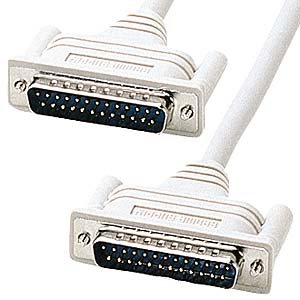
\includegraphics[width=0.35\textwidth]{./img/rs232C}
\caption{RS232C}
%source:http://image.rakuten.co.jp/menet/cabinet/k_02/krs10107k_ma.jpg?_ex=60x60
\label{fig:RS232C}}
\qquad
\begin{minipage}{5cm}
\centering
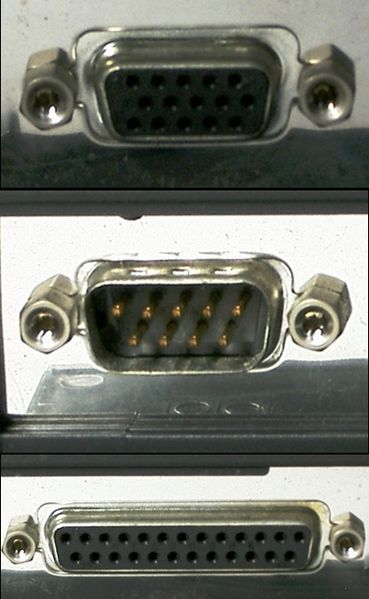
\includegraphics[width=0.7\textwidth]{./img/rs232family}
\caption{RS232family}
%source:https://upload.wikimedia.org/wikipedia/commons/thumb/2/20/VGA-RS-232C-Parallelbus.jpg/369px-VGA-RS-232C-Parallelbus.jpg
\label{fig:RS232Family}
\end{minipage}
\end{figure}
\noindent Złącza typu RS232C można jeszcze spotkać jako interfejs komunikacyjny z drukarkami starego typu, niemniej zostało on wyparty przez nowsze interfejsy (takie jak n.p. USB). \\
\indent Interfejsami najbardziej wydajnymi są USB oraz Ethernet. Są to stosunkowo nowo opracowane (w porównaniu do RS232) i nadal rozwijane interfejsy. Dokładny opis standardu USB znajduje się w rozdziale \ref{USBStandardChapter}. Ethernet jest to ustandaryzowany sposób komunikacji umożliwiający tworzenie komputerowych sieci lokalnych. Początki sięgają roku 1976. Opracowany został w firmie Xerox.
\begin{figure}[H]
\centering
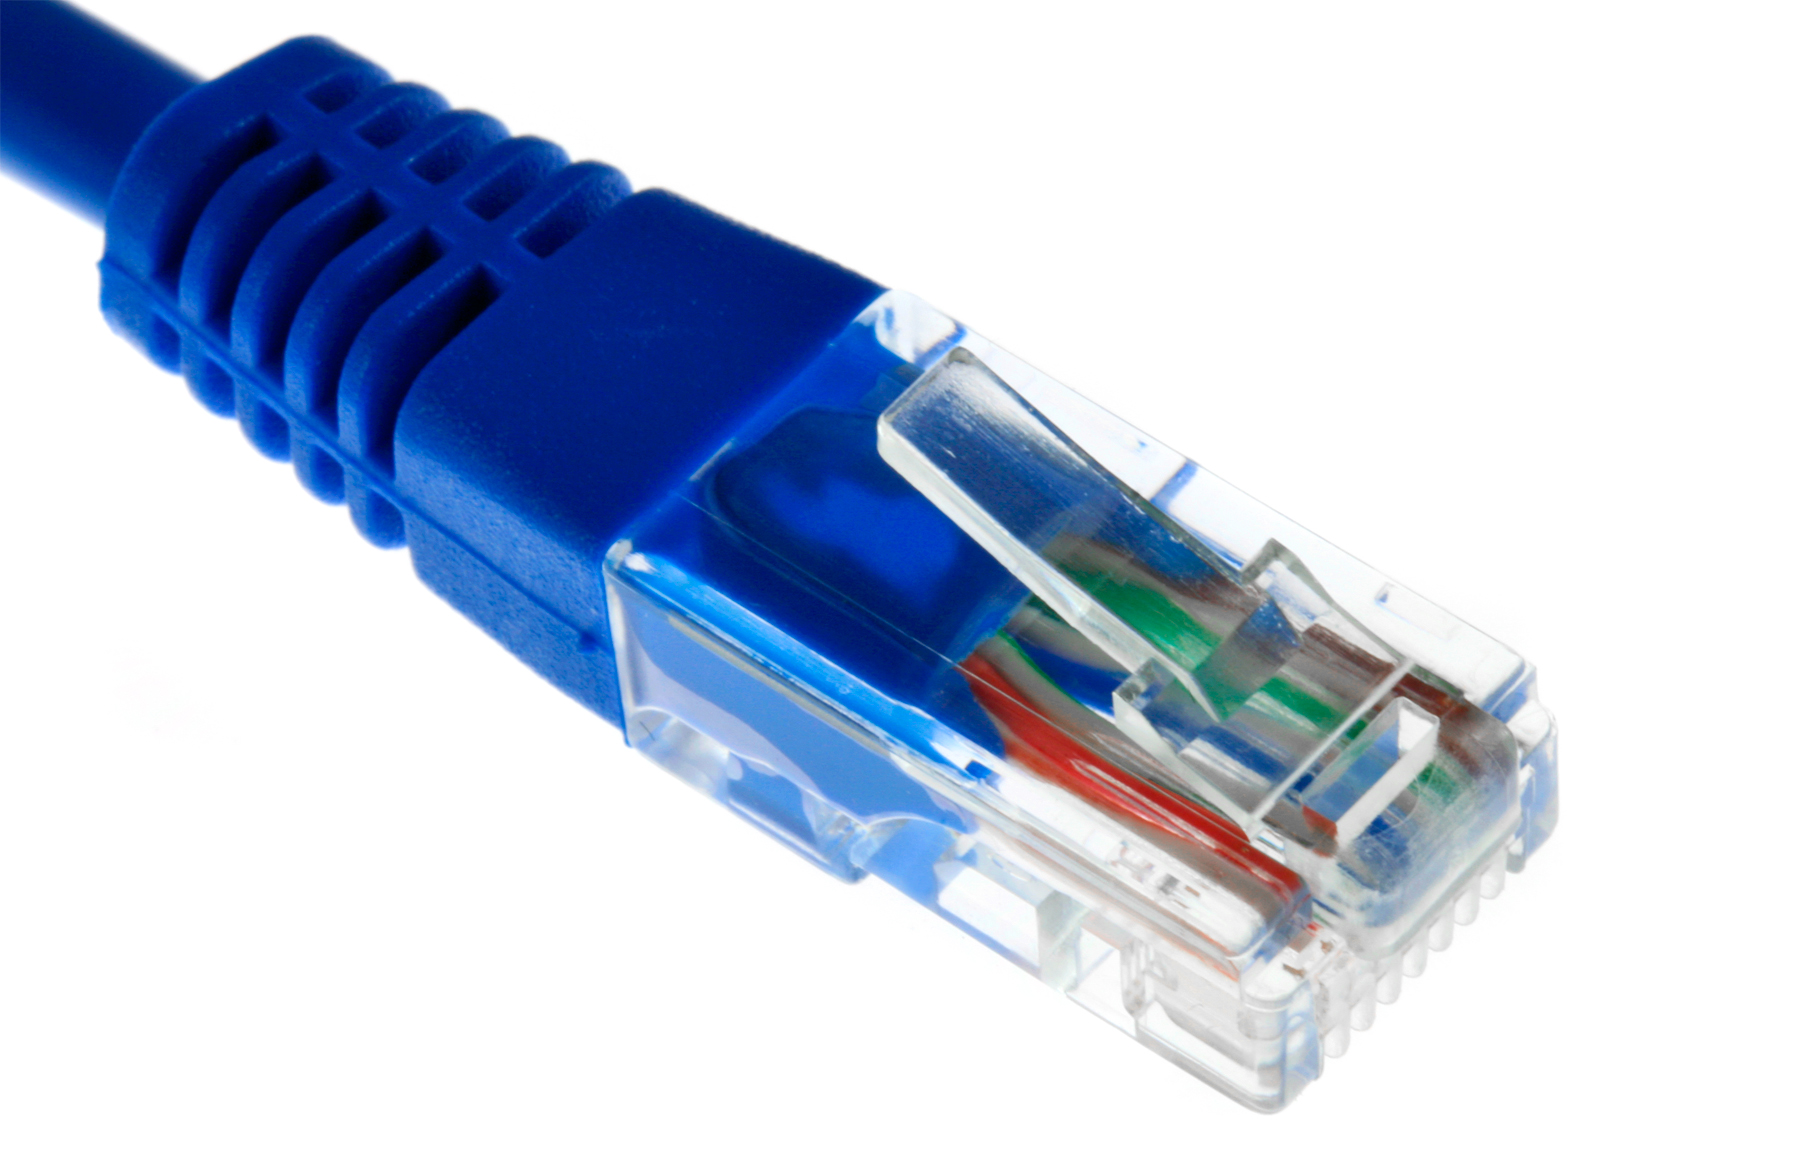
\includegraphics[width=0.35\textwidth]{./img/ethernet-cable}
\caption{EthernetCable}
%source: http://www.av1-ch.com/wp-content/uploads/2014/07/ethernet-cable.jpg
\label{fig:EthernetCable}
\end{figure}
Jeśli chodzi o trudność implementacji to najtrudniejszym do zaimplementowania protokołem/interfejsem przesyłania danych jest Bluetooth. Służy on do bezprzewodowej komunikacji na bardzo krótkim dystansie.
\begin{figure}[H]
\centering

\includegraphics[width=0.35\textwidth]{./img/bluetooth-logo}
\caption{bluetoothLogo}
%source: http://www.theinquirer.net/IMG/177/311177/bluetooth-logo-2-140x227.png?1447285967
\label{fig:blueTooth}
\end{figure}
Dość spotykanym przypadkiem użycia komunikacji bluetooth są zestawy głośno mówiące w samochodach oraz różnego rodzaju urządzenia takie jak słuchawki, głośniki oraz adaptory (np. w zestawie do bezprzewodowej myszki komputerowej dołączany jest adapter bluetooth podpinany pod wejście USB w komputerze).
\newline
\indent Podsumowując, interfejsy szeregowe umożliwiają komunikację miedzy urządzeniami z których jeden najczęściej jest komputerem osobistym. Implementacja każdego interfejsu jest na swój sposób złożona. Kategoryzacja jest możliwa na podstawie różnych wartości. W tym rozdziale zostały podzielone według prostoty interfejsu (w sensie architektury), wydajności oraz trudności implementacji.

\chapter{Czym jest USB}
\label{USBStandardChapter}
Uniwersalna Magistrala Szeregowa jest to standard opracowany w latach 90. XX w. definiujący jakie kable, złącza oraz protokoły mają być używane podczas połączenia, komunikacji oraz definiuje sposób zasilania pomiędzy komputerem i urządzeniem elektronicznym. USB zostało zaprojektowane aby ułatwić połączenia standardowych elektronicznych urządzeń takich jak klawiatury, myszki, drukarki, aparaty cyfrowe, dyski przenośne do komputerów osobistych. Wszystkie te urządzenia są dodatkowo zasilane również za pomocą tego portu. Z czasem stało się to wspólne również dla innych urządzeń takich jak smartphony, palmtopy oraz konsole wideo.\cite{USBSystemArch, USB20Doc, USB30Doc}
\newline
\indent USB szybko zastąpiło porty szeregowe oraz równoległe podobnie jak inne urządzenia zasilające elektroniczne urządzenia.
%%\section{Złącza USB}
\indent Istnieją trzy podstawowe rodzaje złączy USB dla których kryterium podziału stanowi wielkość. Najstarszy rozmiar (używany np. w pendrive'ach) występuje w standardach USB1.1, USB2.0, USB3.0, mini-USB (początkowo tylko dla złącza typu B, jak w wypadku wielu aparatów cyfrowych) oraz mikro-USB występuje również w trzech wariantach dla USB1.1, USB2.0, USB3.0 (dla przykładu używany w nowych telefonach komórkowych). 
\newline
\indent W przeciwieństwie do innych kabli do przesyłu danych (np. Ethernet, HDMI) każdy koniec kabla zakończony jest innym typem złącza (typem A lub typem B). Tylko złącze typu A dostarcza zasilanie. Zostało to zaprojektowane w taki sposób aby uniknąć elektrycznych przeciążeń a co za tym idzie uszkodzeniu urządzeniu. Istnieją również kable ze złączami typu A na obu końcach, ale nie należą do popularnych (i należy postępować z nimi ostrożnie). Kable USB maja zazwyczaj złącze typu A z jednej strony oraz złącze typu B z drugiej oraz wejście w komputerze lub urządzeniu elektronicznym. w przyjętej praktyce złącze typu A jest zazwyczaj największej (z możliwych wielkości), natomiast B w zależności od potrzeb użycia kabla (full, mini, micro). \cite{USBSystemArch, USB20Doc, USB30Doc}

\begin{figure}[h]
\centering
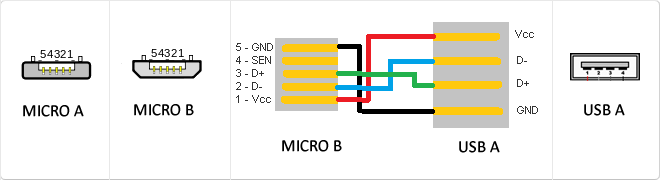
\includegraphics[width=15cm]{./img/micro-usb-type}
\caption{Połączenie przewodów w micro-USB}
\end{figure}
%
% USB ON THE GO ??
%
%%\section{Historia}
\indent USB zapoczątkowało w 1994 siedem firm: Compaq, DEC, IBM, Intel, Microsoft, NEC, Nortel. Celem było uproszczenie podłączenia zewnętrznych urządzeń do komputera zastępując stare złącza w płytach głównych wprowadzając rozwiązania na problemy znalezione w starych oraz upraszczając software.
Pierwszy układ scalony wspierający USB został wyprodukowany przez Intel 1995r.
\newline
%%\subsection{USB1.x}
\indent Pierwsza oficjalna wersja standardu USB została wydana w styczniu 1996r. USB1.0 charakteryzowała prędkość 1,5 Mbit/s (Low Speed) oraz 12 Mbit/s (Full Speed). Nie pozwalał jednak na używanie przedłużaczy kabli, wynikało to z limitów zasilania. %todo: to zdanie nie ma sensu 
Powstało kilka wypuszczono na rynek na chwile przed wydaniem standardu USB1.1 w sierpniu 1998r. W USB1.1 poprawiono kilka błędów znalezionych w USB1.0 i był to pierwszy standard, który został oficjalnie zaimplementowany w standardowych komputerach osobistych. \cite{USBSystemArch}
%%\subsection{USB2.0}
\newline
\indent USB2.0 zostało wydane w kwietniu 2000r. udostępniając maksymalny przesył sygnału rzędu 480 Mbit/s (60MB/s) nazwany High Speed (USB1.x za pomocą Full Speed umożliwiał przesył rzędu 12Mbit/s). Biorąc pod uwagę zależności dostępu do magistrali przepustowość High Speed ogranicza się do 280 Mbit/s (35 MB/s).
Przyszłe modyfikacje do specyfikacji USB zostały zaimplementowane przez "Engineering Change Notitices" (ECN). Najważniejsze z ECNów zostały dołączone do specyfikacji USB2.0 dostępnej na stronie internetowej USB.org.
\newline
Przykłady ECNow:
Złącze Mini-A oraz Mini-B: wydane w październiku 2000r.\cite{USB20Doc}
\newline
%%\subsection{USB3.0}
\indent Standard USB3.0 został wydany w listopadzie 2008r. definiujący zupełnie nowy tryb "SuperSpeed". Port USB zwyczajowo jest w kolorze niebieskim i kompatybilny z urządzeniami USB2.0 oraz kablami.
Dokładnie 17 listopada 2008r. ogłoszono iż specyfikacja dla wersji 3.0 została całkowicie ukończona i została zaakceptowana przez "USB Implementers Forum" (USB-IF), czyli głównej instytucji zajmującej się specyfikacjami standardu USB. To pozwoliło na szybkie udostępnienie standardu deweloperom.
Nowa magistrala "SuperSpeed" dostarcza czwarty typ transferu z możliwością przesyłania sygnału z prędkością 5GBit/s, ale poprzez użycie kodowania 8b/10b przepustowość wynosi 4Gbit/s. Specyfikacja uznaje za zasadne osiągniecie prędkości w okolicach 3,2 Gbit/s (400 MB/s) co w założeniach powinno się zwiększać wraz z rozwijaniem hardwaru. Komunikacja odbywa się w obu kierunkach dla SuperSpeed (kierunek nie jest naprzemienny i nie jest kontrolowany przez hosta, jak to ma miejsce do wersji USB2.0).
Podobnie jak w poprzednich wersjach standardu, porty USB3.0 działają dwóch wariantach zasilania: niskiego poboru mocy (low-power: 150mA) oraz wysokiego poboru mocy (high-power: 900mA). Zapewniając odpowiedni jednocześnie pozwalają na przesył danych z prędkością SuperSpeed.
Została dodatkowo zdefiniowana specyfikacja zasilania (w wersji 1.2 wydana w w grudniu 2010r.) która zwiększała dopuszczalny pobór mocy do 1,5A, ale nie pozwala na współbieżne przesyłanie danych. Specyfikacja wymaga aby fizyczne porty same w sobie były wstanie obsłużyć 5A, ale ogranicza pobór do 1,5 A.
\cite{USB30Doc}
\newline
%\subsection{USB3.1}
\indent W styczniu 2013r. w prasie pojawiły się informacje o planach udoskonalenia standardu USB3.0 do 10Gbit/s. Zakończyło się to stworzeniem nowej wersji standardu - USB3.1. Wersja ta została wydana 31 lipca 2013r. wprowadzając szybszy typ przesyłania danych zwany "SuperSpeed USB 10 Gbit/s". Zaprezentowano również nowe logo stylizowane na zasadzie "Superspeed+". Standard USB3.1 zwiększył szybkość przesyłu sygnału do 10Gbit/s. Udało się też zredukować obciążenie łącza do 3\% dzięki zmianie kodowania na 128b/132b.
\newline
Przy pierwszych testach prędkośi USB3.1 udało się uzyskać prędkość 7,2Gbit/s.
\newline
Standard USB3.1 jest wstecznie kompatybilny ze standardem USB3.0 oraz USB2.0.
\cite{USB30Doc}
\newline
\indent Poszczególne rodzaje kodowania dla standardów USB3.0 oraz USB3.1
%todo later today


\chapter{Biblioteki udostępniające API do komunikacji z USB}
\label{librariesChapter}
Głównym celem projektu jest osiągniecie jak najszybszej prędkości przesyłu danych. Do realizacji celu konieczne jest użycie odpowiedniej biblioteki do komunikacji z interfejsem USB. W rozdziale przedstawiony został krótki opis najbardziej popularnych bibliotek posiadających interfejs komunikacyjny ze złączami USB.
\section{Biblioteka libUSB}
LibUSB jest biblioteką stworzoną w 2007 roku. Napisana w języku C  pozwala na prosty i łatwy dostęp do urządzenia USB. Jest w 100\% przeznaczona dla użytku developera. Biblioteka ma za zadanie ułatwić pisanie aplikacji opartych na komunikacji USB z mikrokontrolerem.
Biblioteka libUSB jest przenośna a co za tym idzie dostępna na wiele platform (Linux, OS X, Windows, Android, OpenBSD, etc.) wraz z niezmiennym API.
Nie są wymagane dodatkowe uprawnienia aby komunikacja z urządzeniem przebiegała poprawnie.
Wspiera standardy USB: 
\begin{itemize}
\item USB1.0 
\item USB1.1 
\item USB2.0 
\item USB3.0
\end{itemize}
Funkcjonalność biblioteki:
\begin{enumerate}
\item wszystkie typy transferu są wspierane (control, bulk, interrupt, isochronous)
\item dwa interfejsy
\begin{enumerate}
\item synchroniczny (prosty)
\item asynchroniczny (bardziej złożony)
\end{enumerate}
\item stosowanie wątków jest bezpieczne
\item lekka biblioteka z prostym API
\item kompatybilna wstecznie (do wersji libUSB-0.1)
\end{enumerate}
(informacje uzyskane dzięki \cite{libusbDesc})
\section{Biblioteka winUSB}
Microsoft Windows począwszy od systemu Windows Vista wprowadził nowy zestaw bibliotek umożliwiający developerom korzystnie z portów USB. WinUSB udostępnia proste API, które pozwala aplikacji na bezpośredni dostęp do portów USB. Został stworzony w gruncie rzeczy dla prostych urządzeń obsługiwanych tylko przez jedną aplikację takich jak urządzenia do odczytu wskaźników pogodowych czy też innych programów które potrzebują szybkiego i bezpośredniego dostępu do portu. WinUSB udostępnia API aby odblokować developera przy pracy z portami USB z poziomu user-mode. W Windowsie 7 USB Media Transfer Protocol (MTP) używa winUSB zamiast poprzednio stosowanych rozwiązań kernela (krenel mode filter driver).

Media Transfer Protocol jest rozszerzeniem PTP (Picture Transfer Protocol) i jest protokołem pozwalającym na przesyłanie atomowe plików audio oraz wideo z oraz do urządzenia. PTP początkowo został zaprojektowany do ściągania zdjęć, obrazów z aparatów cyfrowych, Media Transfer Protocol pozwala na przesyłanie plików muzycznych z cyfrowych urządzeń odtwarzających muzykę oraz pliki video z urządzeń pozwalających na ich odtworzenie.

MTP jest częścią frameworku "Windows Media" blisko związanym z odtwarzaczem Windows Media Player. Systemy Windows począwszy od Windows XP SP2 wspierają MTP. Windows XP wymaga Windows Media Player w wersji 10 lub wyższej, późniejsze wersje systemu wspierają już go domyślnie. Microsoft posiada dodatkowo możliwość zainstalowania MTP na wcześniejszych wersjach systemu ręcznie do wersji Microsoft Windows 98.

Twórcy standardu USB ustandaryzowali MTP jako pełnoprawną klasę dla urządzeń USB w maju 2008r.
Od tamtej pory MTP jest oficjalnym rozszerzeniem PTP i współdzieli ten sam kod klasy. \cite{winusbDesc, micrDevAppUSBDev, micrAccUsbDev, micCommWithUsb}
\newline

%%%\section{Wybór}
\indent Podsumowując w projekcie została użyta biblioteka libUSB. Głównym powodem była możliwość kompilacji programów zarówno pod systemami Unix jak i z rodziny Microsoft Windows bez jakichkolwiek (lub znikomych) zmian w kodzie.

\chapter{Opis zawartości biblioteki libUSB}
\label{libUsbChapter}
\indent Rozdział dokumentujący API używane w projekcie. W rozdziale \ref{librariesChapter} został uzasadniony wybór tej właśnie biblioteki. \cite{libusbDoc}
\section{najważniejsze struktury}
\subsection{libusb\_context}
libusb\_context jest strukturą reprezentującą sesję libusb.
\newline
Koncepcja indywidualnych sesji libusb pozwala aby program mógł korzystać z dwóch bibliotek (lub dynamicznie ładować dwa moduły) z których obie nie zależnie korzystają z libusb. To zapobiega ingerencji (interferencji) pomiędzy dwoma programami używającymi libusb. Dla przykładu libusb\_set\_debug() nie zaingeruje w działanie innego programu korzystającego z libusb, natomiast libusb\_exit() nie wyczyści pamięci używanej przez inny program libusb.
\newline
Sesje tworzone są za pomocą libusb\_init() oraz czyszczone za pomocą libusb\_exit(). Jeśli zagwarantowane jest to, że dana aplikacja jest jedyną która korzysta z libusb, twórca jej nie musi przejmować się kontekstami (strukturą libusb\_context), wystarczy aby przekazywał do wszystkich funkcji, gdzie struktura jest wymagana wartość NULL. Jest to równoważne z użyciem domyślnego kontekstu.

\subsection{libusb\_device\_handle}
Struktura reprezentująca uchwyt do urządzenia USB.
\newline
Jest to nieprzejrzysty typ, użycie jest możliwe tylko za pomocą wskaźnika, zazwyczaj dostarczanego za pomocą funkcji libusb\_open().
\newline
Uchwyt do urządzenia USB jest używany do wykonywania operacji wejścia/wyjścia. Po zakończeniu wszystkich operacji należy wywołać libusb\_close().

\section{najważniejsze funkcje}
\subsection{libusb\_init}
Inicjalizacja biblioteki.
\newline
Funkcja musi zostać wywołana przed wywołaniem jakiejkolwiek innej funkcji z biblioteki libUsb.
\newline
Jeśli w argumencie nie zostanie dostarczony żaden wskaźnik (wyjściowy) kontekstu, zostanie stworzony domyślny kontekst. W przypadku jeśli domyślny kontekst już istnieje zostanie on ponownie użyty (bez ponownej inicjalizacji).
\newline
Funkcja zwraca wartość 0 w wypadku powodzenia, w przeciwnym wypadku zwraca kod błędu.
\subsection{libusb\_open\_device\_with\_vid\_pid}
Wygodna funkcja służąca odszukaniu konkretnego urządzenia na podstawie jego vendorId oraz productId (są to parametry charakteryzujące każde urządzenie).
\newline
Ta funkcja jest używana w przypadkach kiedy z góry jest znane vendorId oraz productId. Najczęściej są to przypadki pisania aplikacji aby przetestować jakąś określoną funkcjonalność. Funkcja pozwala uniknąć wywołanie libusb\_get\_device\_list() i dbania o odpowiednie czyszczenie pamięci po liście.
\newline
Pierwszym parametrem jest kontekst uzyskany za pomocą libusb\_init().
\newline
Kolejnymi parametrami są vendorId oraz productId.
\newline
Funkcja zwraca uchwyt do znalezionego urządzenia, lub NULL w wypadku kiedy nie może znaleźć pożądanego urządzenia (o podanym productId oraz vendorId) lub błędu.
\subsection{libusb\_kernel\_driver\_active}
Funkcja sprawdzająca czy sterownik jądra kernela jest aktywny na interfejsie.
\newline
W wypadku kiedy sterownik jądra jest aktywny nie możliwe jest zgłoszenie użycia interfejsu, a co za tym idzie libUSB nie może wykonać operacji wejścia/wyjścia.
\newline
Funkcjonalność jest nie dostępna w systemie Windows.
\newline
Do funkcji należy przekazać uchwyt do urządzenia oraz numer interfejsu.
\newline
Funkcja zwraca wartość 0, jeśli żaden sterownik jądra nie jest aktywny, wartość 1 w wypadku jeśli istnieje aktywny sterownik jądra.
\newline
W wypadku błędów: LIBUSB\_ERROR\_NO\_DEVICE jeśli urządzenie zostanie odłączone, LIBUSB\_ERROR\_NOT\_SUPPORTED dla platform, gdzie funkcjonalność nie jest wspierana oraz inny kod błędu w wypadku innego błędu.
\subsection{libusb\_detach\_kernel\_driver}
Dzięki funkcji możliwe jest odłączenie sterownika jądra kernela od interfejsu.
\newline
Sukces operacji umożliwi zgłoszenie użycia interfejsu i wykonanie operacji wejścia/wyjścia.
\newline
Funkcjonalność nie jest dostępna dla systemu Windows.
\newline
Parametrami są uchwyt do urządzenia oraz numer interfejsu.
\newline
Funkcja zwraca wartość 0 w momencie powodzenia, LIBUSB\_ERROR\_NOT\_FOUND jeśli żaden sterownik nie był aktywny, LIBUSB\_ERROR\_INVALID\_PARAM jeśli interfejs nie istniej, LIBUSB\_ERROR\_NO\_DEVICE jeśli urządzenie zostało odłączone, LIBUSB\_ERROR\_NOT\_SUPPORTED dla platform, gdzie funkcjonalność nie jest wspierana lub inny kod błędu w wypadku inne błędu.
\subsection{libusb\_claim\_interface}
Dzięki funkcji libusb\_claim\_interface() możliwe jest zgłoszenie użycia danego interfejsu dla danego urządzenia.
\newline
Wywołanie funkcji jest wymagane przed wykonaniem operacji wejścia/wyjścia dla dowolnego punktu końcowego interfejsu.
\newline
Jest dozwolone wywołanie funkcji dla interfejsu już wcześniej zgłoszonego, w tym wypadku zostanie zwrócona wartość 0 bez wykonywania żadnych operacji.
\newline
W wypadku jeśli zmienna auto\_detach\_kernel\_driver jest ustawiona na wartość 1 dla danego urządzenia (zmienna ustawiana za pomocą funkcji: libusb\_set\_auto\_detach\_kernel\_driver()) sterownik jądra zostanie odłączony (jeśli to konieczne), w przypadku niepowodzenia zostanie zwrócony błąd odłączenia.
\newline
Sama procedura wewnątrz funkcji nie jest skomplikowana, nie wymaga wysyłania czegokolwiek po magistrali. Są to proste instrukcje mówiące systemowi operacyjnemu iż aplikacja chce korzystać z danego interfejsu.
\newline
Nie jest to funkcja blokująca.
\newline
Parametrami są uchwyt do urządzenia oraz numer interfejsu zgłaszanego.
\newline
Wartość 0 zostaje zwrócona w wypadku powodzenia operacji.
\newline
W wypadku niepowodzenia kody błędu t.j. LIBUSB\_ERROR\_NOT\_FOUND jeśli podany interfejs nie istnieje, LIBUSB\_ERROR\_BUSY jeśli inny program lub sterownik zarezerwował dany interfejs, LIBUSB\_ERROR\_NO\_DEVICE jeśli urządzenie zostało odłączone oraz inne.
\subsection{libusb\_bulk\_transfer}
Dzięki funkcji możliwy jest przesył większej grupy danych.
\newline
Kierunek jest określony na podstawie bitów kierunkowych punktu końcowego interfejsu.
\newline
Dla odczytu, jeden z parametrów określa ilość danych jaka jest spodziewana przy odczycie. Jeżeli odebrana zostanie mniejsza ilość danych niż oczekiwana, funkcja po prostu zwróci te dane wraz z dodatkowym parametrem określającym ilość otrzymanych danych. Istotne przy odczycie jest to aby sprawdzić czy ilość oczekiwanych danych jest taka jak odczytana.
\newline
W wypadku zapisu również należy sprawdzić czy ilość danych wysłanych pokrywa się z ilością danych skierowaną do wysyłki.
\newline
Wskazana jest również weryfikacja ilości danych wysłanych/odebranych w wypadku wystąpienia timeoutu (funkcja zwróci kod błędu określający timeout). libUSB może podzielić wysyłane dane na mniejsze części i timeout może wystąpić po wysłaniu kilku z nich. Ważne jest to, że nie oznacza to iż nic nie zostało wysłane/odebrane, dlatego należy sprawdzić ilość elementów wysłanych/odebranych i dostosować odpowiednio kolejne kroki.
\newline
Funkcja przyjmuje następujące parametry: uchwyt urządzenia z którym aplikacja będzie się komunikować, adres punktu końcowego interfejsu po którym będzie odbywała się komunikacja, wskaźnik do pamięci danych która ma zostać przetransferowana (w wypadku zapisu) lub odebrana (w wypadku odczytu), ilość danych do wysłania (w przypadku zapisu) lub oczekiwana ilość danych do odebrania (w przypadku odczytu), ilość danych przetransferowanych (w obu przypadkach), maksymalna długość czasu na wykonanie operacji, dla nieograniczonego należy użyć wartości równej 0.
\newline
W przypadku poprawności działania funkcja zwraca wartość 0 oraz ilość przetransferowanych danych przekazanych do funkcji za pomocą wskaźnika.
\newline
W przeciwnym wypadku funkcja zwraca: LIBUSB\_ERROR\_TIMEOUT jeśli transfer przekroczył określony czas, LIBUSB\_ERROR\_PIPE jeśli wystąpił błąd związany z punktem końcowym, LIBUSB\_ERROR\_OVERFLOW jeśli urządzenie wysłało więcej danych niż przewidziane w buforze, LIBUSB\_ERROR\_NO\_DEVICE jeśli urządzenie zostało odłączone oraz inne.
\subsection{libusb\_release\_interface}
Funkcja zwalnia rezerwacje wcześniej zgłoszonego interfejsu za pomocą funkcji libusb\_claim\_interface().
\newline
Zwolnienie wszystkich interfejsów jest wymagane przed zamknięciem urządzenia.
\newline
Nie jest to blokująca funkcja.
\newline
W wypadku jeśli zmienna auto\_detach\_kernel\_driver jest ustawiona na wartość 1 dla danego urządzenia (zmienna ustawiana za pomocą funkcji: libusb\_set\_auto\_detach\_kernel\_driver()) sterownik jądra zostanie ponownie podłączony zaraz po zwolnieniu interfejsu.
\newline
Parametrami są: uchwyt urządzenia oraz numer interfejsu dla niego poprzednio zarezerwowanego.
\newline
Metoda zwraca 0 gdy wszystkie operacje się powiodą.
\newline
W przeciwnym wypadku zwraca: LIBUSB\_ERROR\_NOT\_FOUND jeśli interfejs nie został poprzednio zarezerwowany (zgłoszony do użycia), LIBUSB\_ERROR\_NO\_DEVICE jeśli urządzenie zostało odłączone oraz inne.
\subsection{libusb\_close}
Zwalnia uchwyt do urządzenia.
\newline
Funkcja powinna być wołana na wszystkich używanych uprzednio uchwytach.
\newline
Funkcja pokrótce niszczy referencje stworzoną za pomocą libus\_open() dla danego urządzenia.
\newline
Jest to funkcja nie blokująca.
\newline
Parametrem jest uchwyt przeznaczony do zamknięcia.

\subsection{libusb\_exit}
Funkcja zamyka dostęp do biblioteki.
\newline
Powinna być wołana po zamknięciu wszystkich otwartych urządzeń ale przed zakończeniem działania programu.
\newline
Parametrem jest contekst który ma zostać zamknięty, w wypadku wartości NULL wybierany jest domyślny.

%% asyn interface
\subsection{libusb\_alloc\_transfer}
Funkcja przygotowuje transfer z wyspecyfikowaną ilością 	izochronicznych deskryptorów pakietów.
\newline
Funkcja zwraca uchwyt do zainicjalizowanego transferu. Kiedy wszystkie operacje zostaną na nim wykonane należy wywołać libusb\_free\_transfer().
\newline
Transfer przygotowywany dla nie izochronicznego punktu końcowego należy wywoływać z wartością zero jako ilość izochronicznych pakietów.
\newline
Dla transferów izochronicznych wymagane jest podanie prawidłowej wartości deskryptorów pakietów jakie mają zostać zalokowane w pamięci. Zwracany transfer nie jest domyślnie zainicjalizowany jako izochroniczny, wymagane dodatkowo jest ustawienie pola libusb\_iso\_packets oraz type.
\newline
Alokowanie transferu jako izochroniczny (z podana ilością deskryptorów pakietów do zalokowania) a następnie używanie transferu jako nie izochroniczny jest w 100\% bezpieczne ale pod warunkiem jeśli pole num\_iso\_packets jest ustawione na zero oraz pole type jest ustawione prawidłowo.
\newline
Funkcja jako prametr przyjmuje ilość izochronicznych deskryptorów pakietów.
\newline
Zwracaną jest zalokowany transfer lub NULL w wypadku błędu.
\subsection{libusb\_fill\_bulk\_transfer}
Funkcja pozwala na łatwe przygotowanie struktury libusb\_transfer na transfer masowy.
\newline
Parametrami są:
\begin{itemize}
\item uchwyt do ustawianego transferu
\item uchwyt do urządzenia dla którego ustawiany jest transfer
\item adres punktu końcowego gdzie dane mają zostać wysłane
\item bufor danych do wysłania/odebrania
\item długość (wielkość) wysyłanych/odbieranych danych
\item wskaźnik do funkcji która ma się wywołać po zakończeniu transferu (callback)
\item dodatkowe dane, które programista może opcjonalnie wysłać do funkcji wywołanej po zakończeniu transferu 
\item czas oczekiwania w milisekundach na zakończenie transferu
\end{itemize}
\subsection{libusb\_submit\_transfer}
Funkcja wykonuje podany (ustawiony) transfer.
\newline
Funkcja wykonuje operacje na interfejsie po czym bezzwłocznie kończy działanie.
\newline
Jedynym parametrem jaki przyjmuje funkcja jest wskaźnik do transferu jaki ma zostać wykonany.
\newline
W wypadku kiedy wszystko się powiedzie funkcja zwraca wartość równą 0, w pozostałych przypadkach zwraca kod błędu tj. LIBUSB\_ERROR\_NO\_DEVICE w wypadku kiedy urządzenie nie jest podłączone, LIBUSB\_ERROR\_BUSY w przypadku jeśli akcja została już wykonana, LIBUSB\_ERROR\_NOT\_SUPPORTED jeśli flagi transferu (ustawienia) są nie wspierane przez system operacyjny oraz inne.
\subsection{libusb\_free\_transfer}
Funkcja odpowiada za zwolnienie pamięci zajętą przez strukturę libusb\_transfer
\newline
Funkcja ta powinna być zawołana dla wszystkich transferów zaalokowanych przez libus\_alloc\_transfer().
\newline
Jeśli dodatkowo flaga LIBUSB\_TRANSFER\_FREE\_BUFFER jest ustawiona oraz bufor transferu jest nie zerowy, pamięć po nim zostanie również zwolniona za pomocą standardowej funkcji alokującej (np. free()).
\newline
Dozwolone jest zawołanie funkcji z parametrem równym NULL, w takim przypadku funkcja zakończy się bez błędu (ale nic nie zostanie zwolnione).
\newline
Nie dozwolone jest zwalnianie pamięci po nie zakończonym (aktywnym) jeszcze transferze, czyli takim który wystartował ale jeszcze nie wywołany został callback do niego (lub timeout).
\newline
Parametrem funkcji jest wskaźnik do transferu do zwolnienia.

%---------
\chapter{Urządzenie testowe}
\label{microcontrollerChapter}
Aby zrealizować projekt konieczne było użycie dodatkowego hardwaru, którego zadaniem było odbieranie danych po przeciwnej stronie jak i przesył w drugą stronę. Inwestygacja rozpoczęła się od bardzo prostych urządzeń takich jak raspberry pi B+, a zakończyła się na mikrokontrolerze LandTiger.

\begin{figure}[h]
\centering
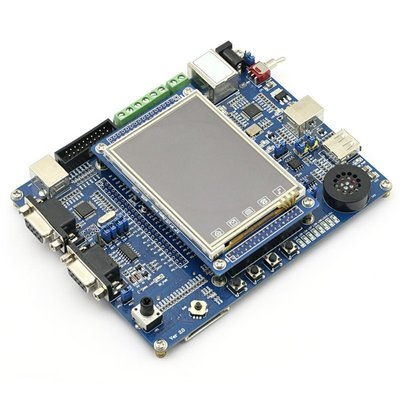
\includegraphics{./img/landTiger}
\caption{Mikrokontroler LandTiger wraz z wyświetlaczem}
\end{figure}

Mikrokontroler LandTiger oparty na LPC1768 został wyprodukowany przez firmę PowerMCU i można ją zakupić od wielu dostawców na eBay lub innych serwisach świadczących usługi zakupów przez internet. Średni koszt waha się w granicach \$70 za płytkę wraz z wyświetlaczem LCD 3,2 cala o rozdzielczości 320x240 pikseli, z zasilaczem oraz zestawem kabli. \cite{landtigerDesc}
\newline
Funkcjonalności:
\begin{enumerate} [label=(\alph*)]
\item 2 porty RS232, jeden z nich wspiera ISP (In-system Programming)
\item 2 interfejsy magistrali CAN (Controller Area Network)
\item interfejs RS485
\item interfejs Ethernetowy RJ45-10/100M 
\item przetwornik cyfrowo-analogowy (DAC) wraz wmontowanym głośnikiem (wyjściem interfejsu) oraz sterownikiem dźwięku (LM386)
\item przetwornik analogowo-cyfrowy (ADC) wraz z wbudowanym potencjomentrem (wejściem interfejsu).
\item Kolorowy 3,2 cala (lub 2,8 cala) dotykowy wyświetlacz LCD o rozdzielczości 320x240 pikseli. 
\item interfejs USB2.0 (USB Host oraz USB Device)
\item interfejs kard SD/MMC
\item interfejs I2C połączony z 2Kbit pamięcią EEPROM
\item interfejs SPI połączony z 16Mbit pamięcią flash
\item 2 user keys, 2 function keys
\item 8 diód typu LED
\item pięciokierunkowy joystick
\item wsparcie dla pobierania ISP
\item pobieranie z użyciem JTAG, interfejs dla debugowania
\item zintegrowany emulator kompilacji JLINK - wspiera możliwość debugownia online (po kablu USB podłączonym do PC) dla środowisk deweloperskich tj. KEIL, IAR, CooCox i innych
\item dodatkowe 5V port zasilający (możliwe jest też za pomocą portu USB 
\end{enumerate}

\begin{figure}[h]
\centering
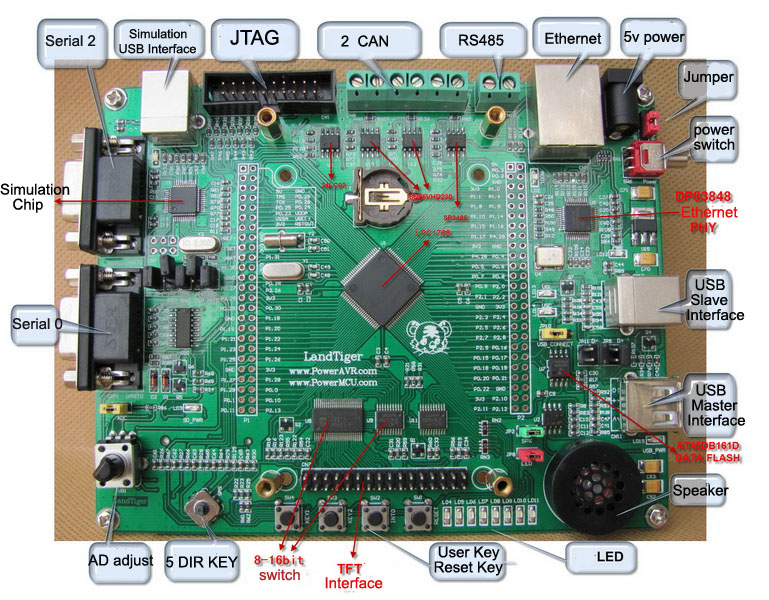
\includegraphics{./img/landTiger3}
\caption{Mikrokontroler LandTiger wraz z opisem poszczególnych elemetnów}
%example\caption{Krzywa plastyczności wyrażająca zależność odkształcenia od naprężenia podczas rozciągania materiału ciągliwego \cite{bib7}} 
\end{figure}
LandTiger jest oparty na LPC1768. Wbudowany hardware wspiera ISP aby umożliwić załadowanie kodu (z użyciem bin2hex oraz flashmagic).
\newline
Alternatywą jest to, że kod może zostać załadowany za pomocą emulatora JLINK JTAG/SWD lub za pomocą zewnętrznego urządzenia JTAG.
\newline
Port COM1 (UART0) wspiera komunikacje z PC w obie strony. Wszelkie funkcje portu USB są wspierane z minimalnymi zmianami w oprogramowaniu. Podobnie jest z Ethernetem, z niewielkimi  zmianami w oficjalnym kodzie dla LPC1768 kod jest w stanie się uruchomić na LandTigerze.
\newline
\indent Wyświetlacz LCD jest oparty na kontrolerze SSD1289. Wyświetlacz może zostać odłączony od płyty. Używa 8-bitowej magistrali \(P2_0..P2_7\). Kontroler ekranu dotykowego jest dostarczony razem z modułem wyświetlacza. Interfejs pomiędzy ekranem dotykowym a LPC1768 jest możliwy dzięki SPI.
\newline
Główne różnice pomiędzy LandTigerem a LPC1768:
\begin{enumerate} [label=(\alph*)]
\item płyta po podłączeniu do PC nie pokazuje się jako zewnętrzne urządzenie magazynujące
\item aby ściągnąć nowe pliki binarne należy użyć ISP lub JTAG
\item brak wsparcia dla serialowego portu po linku USB, należy używać RS232 lub portu USB
\item brak wsparcia dla logicznego systemu plików
\item brak wsparcia dla 4 diód typu LED (istnieje możliwość użycia inncyh).
\end{enumerate}

Parametry mikrokontrolera LandTiger wydawały się być zadowalające aby wykonać na nim testy. Niestety jak się podczas egzekucji testów okazało (a zostało dokładniej opisane w rozdziale \ref{resultsChapter}) pomimo wlutowanego złącza USB wspierającego USB2.0 chip na kontrolerze wspiera standard USB1.1. Dzięki wynikom uzyskanym z użyciem LandTiger'a możemy obliczyć możliwości gdyby wsparcie USB2.0 na kontrolerze było zaimplementowane.


\iffalse
%% not inluded into pdf right now
\chapter{Synchroniczne przesyłanie danych}
\label{synchronicChapter}
Jedną z metod dostępnych, która została użyta w przygotowaniu tej pracy jest wykorzystanie synchronicznych możliwości przesyłu danych z wykorzystaniem libUSB.

\section{zalety}
\begin{itemize}
\item duża kontrola nad wysyłanymi/odbieranymi danymi
\item debugowanie jest mało skomplikowane w porównaniu do asynchronicznego przesyłania danych
\end{itemize}
\section{wady}
\begin{itemize}
\item możliwości prędkości są mocno ograniczone poprzez funkcje blokujące
\end{itemize}
\fi



\chapter{Implementacja}
\label{implementationChapter}
Implementacja opiera się na wykorzystaniu prostych podstawowych funkcji z biblioteki libUsb. Rozwiązania zostały obudowane w odpowiednie klasy wraz z zastosowaniem polimorfizmu aby uzyskać możliwość łatwego dodawania nowych udoskonaleń.

\section{Klasa Mode}
Klasa Mode jest nadzbiorem funkcjonalności. Klasa ta obudowuje podstawowe funkcjonalności takie jak:
\begin{itemize}
\item inicjalizacja
\subitem pobieranie kontekstu
\subitem pobieranie uchwytu urządzenia
\subitem rejestracja interfejsu
\item oczyszczanie pamięci
\end{itemize}
Klasa zawiera również czysto wirtualną metodę doTest(), której odpowiednie implementacje w klasach dziedziczących dostarcza funkcjonalności testom.
\begin{lstlisting}[caption={Deklaracja klasy Mode},label={lst:CMode}]
class Mode
{
public:
	Mode(int bufforSize, unsigned count, int vid, int pid, bool printOnlyResult) : _bufforSize(bufforSize), _count(count), _vid(vid), _pid(pid), _printOnlyResult(printOnlyResult)
	{
		_debugPrinter.set(!printOnlyResult);
	}
	virtual ~Mode();
	virtual int generateSymulatedData(unsigned char*, const int);
	virtual void printFinalInformation();
	virtual void initProcedures();
	virtual void getContext();
	virtual void getDeviceHandle();
	virtual void proceedWithInitUsb();
	virtual void closeLibUsb();
	virtual int doTest() = 0;
	
protected:
	int _bufforSize;
	unsigned _count;
	int _vid;
	int _pid;
	double _timeResult;
	DebugPrinter _debugPrinter;
	bool _printOnlyResult;
	libusb_context* _ctx;
	libusb_device_handle* _dev_handle;

};
\end{lstlisting}
\subsection{Metoda getContext}
W listingu \ref{lst:Mode_getContext} przedstawione zostało ciało metody getContext() klasy Mode.
\newline
Metoda nie przyjmuje żadnego argumentu, natomiast inicjalizuje kontekst i zapamiętuje go jako składnik w składowej klasy. W rozdziale \ref{libUsbChapter} wspomniane zostało iż możliwe jest używanie kontekstu domyślnego, wtedy zamiast użycia libusb\_init() należałoby przypisać wskaźnikowi do kontekstu wartość równą NULL. 
\newline
Aby używać domyślnego kontekstu należy mieć pewność iż aplikacja/wątek jest jedynym użytkownikiem libUSB.
\newline
W wypadku niepoprawnego działania wyrzucany jest błąd (ważne aby był przechwycony w funkcji main).
\begin{lstlisting}[caption={Metoda Mode::getContext()},label={lst:Mode_getContext}]
void Mode::getContext()
{	
	int r = libusb_init(&_ctx);
	if(r < 0) {
		throw std::runtime_error("Init Context error");

	}
}
\end{lstlisting}
\subsection{Metoda getDeviceHandler}
Metoda nie przyjmuje żadnego argumentu. Ustawiany jest uchwyt do urządzenia na podstawie jego vendorId oraz productId (testy były wykonane na mikrokontrolerze LandTige). W wypadku niepowodzenia zostanie zgłoszony odpowiedni błąd (np. braku podłączonego i uruchomionego mikrokontrolera).
Ciało funkcji zostało przedstawione w Listingu \ref{lst:Mode_getDeviceHandle}
\begin{lstlisting}[caption={Metoda Mode::getDeviceHandler()},label={lst:Mode_getDeviceHandle}]
void Mode::getDeviceHandle()
{
	_dev_handle = libusb_open_device_with_vid_pid(_ctx, _vid, _pid);
	if(_dev_handle == NULL)
		throw std::runtime_error("Cannot open device!");
	else
		_debugPrinter << "Device Opened\n";
}
\end{lstlisting}
\subsection{Metoda proceedWithInitLibUsb}
Metoda odpowiedzialna za dokończenie procedur inicjalizacyjnych. Ciało metody zostało przedstawione w Listingu \ref{lst:Mode_proceedWithInitLibUsb}. Metoda sprawdza dodatkowo czy sterownik jądra kernela jest aktywny, dla platformy Windows funkcja zwróci wartość LIBUSB\_ERROR\_NOT\_SUPPORTED (!= 1) i zachowa się analogicznie jak w wypadku nie aktywnego sterownika w systemie UNIX (warunek bedzie nie spełniony).
\newline
Kolejnym krokiem jest rezerwacja przez program konkretnego interfejsu za pomocą funkcji libusb\_claim\_interface.
\newline
W wypadku niepoprawnego działania metoda wyrzuci runtime\_error który należy obsłużyć  w funkcji main().
\begin{lstlisting}[caption={Metoda Mode::proceedWithInitLibUsb()},label={lst:Mode_proceedWithInitLibUsb}]
void Mode::proceedWithInitUsb()
{
	if(libusb_kernel_driver_active(_dev_handle, 0) == 1) { //find out if kernel driver is attached
		_debugPrinter << "Kernel Driver Active\n";
		if(libusb_detach_kernel_driver(_dev_handle, 0) == 0) //detach it
			_debugPrinter << "Kernel Driver Detached!\n";
	}
	int status = libusb_claim_interface(_dev_handle, 1);
	if(status < 0) 
	{
		throw std::runtime_error("Cannot Claim Interface");
	}
	_debugPrinter << "Claimed Interface\n";
}
\end{lstlisting}

\subsection{Metoda initProcedures()}
Metoda przedstawiona w listingu \ref{lst:Mode_initProcedures} odpowiada za wywołanie procedur inicjalizacji w odpowiedniej kolejności.
\begin{lstlisting}[caption={Metoda Mode::initProcedures()},label={lst:Mode_initProcedures}]
void Mode::initProcedures()
{
	getContext(); 
	getDeviceHandle();
	proceedWithInitUsb();
}
\end{lstlisting}
\subsection{Metoda closeLibUsb}
Metoda przedstawiona w Listingu \ref{lst:Mode_closeLibUsb} odpowiada za zwolnienie interfesju oraz zasobów uprzednio zajętych na czas testu.
\begin{lstlisting}[caption={Metoda Mode::closeLibUsb()},label={lst:Mode_closeLibUsb}]
void Mode::closeLibUsb()
{
	int status = libusb_release_interface(_dev_handle, 1); 
	if(status != 0) {
		throw std::runtime_error("Cannot Relase Interface");
	}
	_debugPrinter << "Released Interface\n";
	libusb_close(_dev_handle);
	libusb_exit(_ctx); 
}
\end{lstlisting}


\subsection{Metoda printFinalInformation}
Metoda mająca na zadanie wypisanie ostatecznych wyników. Wyniki mogą zostać przedstawione jako czytelna zwykła informacja dla użytkownika lub w postaci kolumnowej (używanej przy tworzeniu wykresów).
\begin{lstlisting}[caption={Metoda Mode::printFinalInformation()},label={lst:Mode_printFinalInformation}]
void Mode::printFinalInformation()
{
	_debugPrinter << "Sending of: " << _bufforSize * _count << "Bytes using bufferSize=" << _bufforSize << " takes " << _timeResult << "s.\n";
	if(_printOnlyResult)
	{
		unsigned allSendReceivedData = _bufforSize * _count;
		double sendingTime = _timeResult/2;
		double receivingTime = _timeResult/2;

		printf("%d\t%u\t%u\t%.2f\t%.2f\t%.2f\t%.2f\t%.2f\t%.2f\n", _bufforSize, _count, allSendReceivedData, _timeResult, sendingTime, receivingTime,
							allSendReceivedData/_timeResult, allSendReceivedData/sendingTime, allSendReceivedData/receivingTime);
	}
}
\end{lstlisting}
\section{Klasa SynchMode}
Klasa SynchMode odpowiada odpowiednią konfigurację USB dla przesyłu synchronicznego. 

\begin{lstlisting}[caption={Deklaracja klasy SynchMode},label={lst:CSynchMode}]
class SynchMode : public Mode
{
public:
	SynchMode(int bufforSize, unsigned count, int vid, int pid, bool printOnlyResult);
	virtual ~SynchMode();
	virtual int doTest() override;

private:

};
\end{lstlisting}
Klasa używa wszystkich domyślnych ustawień (nie przeciąża żadnej metody wirtualnej), oczywiście metoda doTest() wymaga implementacji.
\subsection{Metoda doTest}
Metoda w całości przedstawiona w listingu \ref{lst:SynchMode_doTest} i jest odpowiedzialna za wykonanie podstawowego pomiaru czasu przepływu danych w obie strony pomiędzy PC a mikrokontrolerem.
\newline
Została zaprojektowana w taki sposób aby konkretny bufor danych został wysłany oraz odebrany określoną ilość razy i zwrócony przedział czasowy w jakim udało się to uzyskać. Powodem wysyłania/odbierania danych określoną ilość razy jest fakt dość sporych ograniczeń jeśli chodzi o chip wbudowany w płytę LandTiger.
\begin{lstlisting}[caption={Metoda SynchMode::doTest()},label={lst:SynchMode_doTest}]
int SynchMode::doTest()
{
	unsigned char *data_out = new unsigned char[_bufforSize]; //data to write
	unsigned char* data_in = new unsigned char[_bufforSize];
	generateSymulatedData(data_out, _bufforSize);
	int howManyBytesIsSend; 
	int howManyBytesReceived;

	time_t start_t, end_t;
    	_timeResult = 0;

	
	time(&start_t);
	for(int i = 0; i < _count; ++i)
	{
		int sendStatus = libusb_bulk_transfer(_dev_handle, (2 | LIBUSB_ENDPOINT_OUT), data_out, _bufforSize, &howManyBytesIsSend, 0); 
		if(sendStatus == 0 && howManyBytesIsSend == _bufforSize)
		{
			//here was printing data for debugging only
		}
		else
		{
			delete [] data_out;
			throw std::runtime_error("Write Error!");
		}
		
		
		int readStatus = libusb_bulk_transfer(_dev_handle, (2 | LIBUSB_ENDPOINT_IN), data_in, _bufforSize * sizeof(unsigned char), &howManyBytesReceived, 0);
		if (readStatus == 0 && howManyBytesReceived == howManyBytesIsSend) 
		{
			//here was printing data for debugging only
		} 
		else 
		{
			delete[] data_in;
			throw std::runtime_error("Read Error! ");
		}
		
	}
	time(&end_t);
	_timeResult = difftime(end_t, start_t);
	delete[] data_in;
	delete [] data_out;
	return 0;
}
\end{lstlisting}
\section{Klasa AsynchMode}
Klasa AsynchMode odpowiada odpowiednią konfigurację USB dla przesyłu asynchronicznego. 

\begin{lstlisting}[caption={Deklaracja klasy SynchMode},label={lst:CAsynchMode}]
class AsynchMode : public Mode
{
public:
	AsynchMode(int bufforSize, unsigned count, int vid, int pid, bool printOnlyResult);
	virtual ~AsynchMode();
	virtual int doTest() override;
	virtual void initProcedures() override;
	void closeLibUsb() override;
private:
	pthread_mutex_t _sender_lock;
	pthread_mutex_t _receiver_lock;
	pthread_cond_t _sender_cond;
	pthread_cond_t _receiver_cond;

	libusb_transfer* _senderTransfer;
	libusb_transfer* _receiverTransfer;
	pthread_t _receiverThread;

};
\end{lstlisting}
Klasa zawiera wzbogaconą inicjalizację o alokacje transferów (wysyłającego oraz odbierającego) oraz inicjalizację mutexów.
\newline
Dosyć istotnym elementem jest przedstawiony w listingu \ref{lst:ThreadHelper} dodatkowy namespace ułatwiający obsługę callbacków. Znajduje się w nim zarówno obsługa wątku nasłuchującego jak i obsługa poszczególnych zdarzeń.
\begin{lstlisting}[caption={Deklaracja klasy SynchMode},label={lst:ThreadHelper}]
namespace ThreadHelper
{
	struct TransferStatus
	{
		time_t startTest;
		time_t stopTest;
		int allCompleted;
		libusb_transfer* senderHandler;
		libusb_transfer* receiverHandler;
		int sendCount;
		int receivedCount;
		int needToBeSendReceived;
		libusb_context* ctx;
		int waitForSender;
		int waitForReceiver;
		int particularSendComplete;
		int particularReceiveComplete;
		pthread_mutex_t* sender_lock;
		pthread_mutex_t* receiver_lock;
		pthread_cond_t* sender_cond;
		pthread_cond_t* receiver_cond;
	};

	static void LIBUSB_CALL cb_read(struct libusb_transfer *transfer)
	{
		if (transfer->status != LIBUSB_TRANSFER_COMPLETED) {
			std::cerr << "Reading data error!" << std::endl;
			return ;
		}
		TransferStatus* ts = static_cast<TransferStatus*>(transfer->user_data);
		ts->receivedCount++;
		ts->particularReceiveComplete = 1;
	
		pthread_mutex_lock(ts->sender_lock);
		ts->waitForSender = 0;
		pthread_cond_signal(ts->sender_cond);
		pthread_mutex_unlock(ts->sender_lock);
		if(ts->receivedCount == ts->needToBeSendReceived)
		{
			time(&ts->stopTest);
			ts->allCompleted = 1;
		}

	}

	static void LIBUSB_CALL cb_send(struct libusb_transfer *transfer)
	{
		if (transfer->status != LIBUSB_TRANSFER_COMPLETED) {
			std::cerr << "Sending data error!" << std::endl;
			return ;
		}
		TransferStatus* ts = static_cast<TransferStatus*>(transfer->user_data);
		ts->sendCount++;
		pthread_mutex_lock(ts->receiver_lock);
		ts->waitForReceiver = 0;
		ts->particularSendComplete = 1;
		pthread_cond_signal(ts->receiver_cond);
		pthread_mutex_unlock(ts->receiver_lock);

	}
	
	void* receiverThread(void* arg)
	{
		TransferStatus* transferStatus = static_cast<TransferStatus*>(arg);
		while(transferStatus->allCompleted != 1) 
		{
			pthread_mutex_lock(transferStatus->receiver_lock);
			while(transferStatus->waitForReceiver) {
				pthread_cond_wait(transferStatus->receiver_cond, transferStatus->receiver_lock);
			}
			transferStatus->waitForReceiver = 1;

			pthread_mutex_unlock(transferStatus->receiver_lock);
			transferStatus->particularReceiveComplete = 0;
			libusb_submit_transfer(transferStatus->receiverHandler);
			while(transferStatus->particularReceiveComplete == 0)
				libusb_handle_events(transferStatus->ctx);
		}
	}

}
\end{lstlisting}
\subsection{Metoda initProcedures oraz closeLibUsb}
W wypadku Asynchronicznego przesyłania danych należy wykonać kilka dodatkowych operacji inicjalizacyjnych. Są to alokacje transferów oraz inicjalizacja mutexów.
Calość widoczna w listingu \ref{AsynchMode_initProcedures}.
\begin{lstlisting}[caption={Metoda AsynchMode::initProcedures},label={lst:AsynchMode_initProcedures}]
void AsynchMode::initProcedures()
{
	Mode::initProcedures();
	_senderTransfer = libusb_alloc_transfer(0);	
	_receiverTransfer = libusb_alloc_transfer(0);
	if(_senderTransfer == NULL || _receiverTransfer == NULL)
	{
		throw std::runtime_error("Transfer allocation Error");
	}

	if(pthread_mutex_init(&_sender_lock, NULL) != 0 || pthread_mutex_init(&_receiver_lock, NULL) != 0)
	{
		throw std::runtime_error("Mutex Init Failed!");
	}

}
\end{lstlisting}
Analogicznie sytuacja przedstawia się sytuacja w wypadku zwalniania zasobów. Dodatkową czynnością jest usunięcie mutexów oraz zwolnienie transferów. Całość dostępna w listingu \ref{lst:AsynchMode_closeLibUsb}.
\begin{lstlisting}[caption={Metoda AsynchMode::closeLibUsb},label={lst:AsynchMode_closeLibUsb}]
void AsynchMode::closeLibUsb()
{
	pthread_mutex_destroy(&_sender_lock);
	pthread_mutex_destroy(&_receiver_lock);
	libusb_free_transfer(_senderTransfer);
	libusb_free_transfer(_receiverTransfer);
	Mode::closeLibUsb();
}
\end{lstlisting}
\subsection{Metoda doTest}
Podobnie jak w wypadku Synchronicznego mechanizmu tak i teraz należy dostarczyć implementacje metody doTest(). Jej działanie jest znacznie odmienne, polega na wystartowaniu drugiego wątku nasłuchującego odpowiedzi. Całość synchronizowana jest za pomocą mutexów (listing \ref{lst:AsynchMode_doTest} oraz \ref{lst:ThreadHelper}).
\begin{lstlisting}[caption={Metoda AsynchMode::doTest()},label={lst:AsynchMode_doTest}]
int AsynchMode::doTest()
{
	unsigned char *data_out = new unsigned char[_bufforSize]; //data to write
	unsigned char *data_in = new unsigned char[_bufforSize]; //data to read
	generateSymulatedData(data_out, _bufforSize);
	int howManyBytesIsSend; 
	int howManyBytesReceived;
	ThreadHelper::TransferStatus transferStatus;
	transferStatus.allCompleted = 0;
	
	transferStatus.sendCount = 0;
	transferStatus.receivedCount = 0;
	transferStatus.senderHandler = _senderTransfer;
	transferStatus.receiverHandler = _receiverTransfer;
	transferStatus.needToBeSendReceived = _count;
	transferStatus.ctx = _ctx;
	transferStatus.waitForSender = 0;
	transferStatus.waitForReceiver = 1;
	transferStatus.sender_lock = &_sender_lock;
	transferStatus.sender_cond = &_sender_cond;
	transferStatus.receiver_lock = &_receiver_lock;
	transferStatus.receiver_cond = &_receiver_cond;
	
	libusb_fill_bulk_transfer(_senderTransfer, _dev_handle, (2 | LIBUSB_ENDPOINT_OUT), data_out, _bufforSize, ThreadHelper::cb_send, &transferStatus, 0);
	libusb_fill_bulk_transfer(_receiverTransfer, _dev_handle, (2 | LIBUSB_ENDPOINT_IN), data_in, _bufforSize, ThreadHelper::cb_read, &transferStatus, 0);

	_timeResult = 0.0;
	if(pthread_create(&_receiverThread, NULL, ThreadHelper::receiverThread, &transferStatus) != 0)
	{
		throw std::runtime_error("Error creating listener thread.");
	}
	
	time(&transferStatus.startTest); 
	for(int i = 0; i < _count; ++i)
	{
		pthread_mutex_lock(&_sender_lock);
		while(transferStatus.waitForSender){
			pthread_cond_wait(&_sender_cond, &_sender_lock);
		}
		transferStatus.waitForSender = 1;

		pthread_mutex_unlock(&_sender_lock);
		transferStatus.particularSendComplete = 0;
		libusb_submit_transfer(_senderTransfer);
		while(transferStatus.particularSendComplete == 0)
			libusb_handle_events(_ctx);
		
	}
	pthread_join(_receiverThread, NULL);
	_timeResult = difftime(transferStatus.stopTest, transferStatus.startTest);
	delete data_out;
	delete data_in;
	return 0;
}

\end{lstlisting}

\section{Korzystanie z poszczególnych interfejsów}
Kod przedstawiony w Listingu \ref{lst:main} doskonale ukazuje prostotę korzystania z libUSB. Użytkownik zobligowany jest do wprowadzenia wielkości bufora danych oraz ilości powtórzeń określających ile razy dany bufor zostanie wysłany do mikrokontrolera. Następnie zostaje wykonana inicjalizacja z użyciem wyżej wymienionych interfejsów (synchronicznego lub asynchronicznego na podstawie parametru).
\begin{lstlisting}[caption={Przykład użycia interfejsu synchronicznego lub asynchronicznego w zależności od parametryzacji},label={lst:main}]
int main(int argc, char* argv[])
{
	
	if(argc < 4) 
	{
		std::cout << "use: " << argv[0] << " [S/A] <bufforSize> <fullDataSize> optional:<printOnlyResult>" << std::endl;
		std::cout << "First parameter tells if application should be run in Synchronous mode or Asynchronous" << std::endl;
		std::cout << "Note that max buffer of LandTiger is " << BUFFOR_MAX << "Bytes" << std::endl;
		return 0; 
	}
	bool printOnlyResult = false;
	if(argc == 5)
		printOnlyResult = argv[4][0] == '0' ? false : true;
	
	DebugPrinter debugPrinter(! printOnlyResult);
	char selectedMode = std::toupper(argv[1][0]);
	if(selectedMode != 'A' && selectedMode != 'S')
	{
		debugPrinter << "mode set is different than A or S, setting synchronous as default.\n";
		selectedMode = 'S';
	}
		
	unsigned bufforSize = atoi(argv[2]);
	if(bufforSize > BUFFOR_MAX) 
	{
		debugPrinter << "bufforSize is grather than 64B, setting 64 as default\n";
		bufforSize = BUFFOR_MAX;
	}
	unsigned fullDataSize = atoi(argv[3]);
	unsigned count = fullDataSize/bufforSize;
	if(fullDataSize % bufforSize != 0)
	{
		debugPrinter << "It is impossible to send " << fullDataSize << "B using " << bufforSize << "B, to simplify application work sending " << (++count) * bufforSize << "B\n";
	}
	

	debugPrinter << "Total size to send/receive: " << bufforSize << " x " << count << " = " << bufforSize * count << " Bytes\n";
	try 
	{
		std::unique_ptr<Mode> mode;

		if(selectedMode == 'A')
			mode.reset(new AsynchMode(bufforSize, count, LAND_TIGER_VID, LAND_TIGER_PID, printOnlyResult));
		else 
			mode.reset(new SynchMode(bufforSize, count, LAND_TIGER_VID, LAND_TIGER_PID, printOnlyResult));
		mode->initProcedures();
		mode->doTest();
		mode->printFinalInformation();
		mode->closeLibUsb();
	} catch (std::runtime_error& e)
	{
		std::cout << e.what() << std::endl;
	}

	return 0;
}

\end{lstlisting}
\subsection{Parametryzacja}
\begin{lstlisting}[caption={uruchomienie testu}]
use: libusb [S/A] <bufforSize> <fullDataSize> optional:<printOnlyResult>
\end{lstlisting}
\begin{itemize}
\item S/A - należy wybrać czy chcemy wykonać test w trybie Synchronicznym czy Asynchronicznym
\item bufforSize - rozmiar bufforu danych jaki chcemy przeznaczyć dla jednej paczki danych [B]
\item fullDataSize - całkowity rozmiar danych do wysłania [B]
\item printOnlyResult - opcjonalny parametr w wypadku ustawienia na wartość '1' pozwala na łatwe zebranie wyników bez zbędnych informacyjnych wiadomości (same dane). 
\end{itemize}
\section{embedded code}
Po stronie mikrokontrolera LandTiger konieczne było zaimplementowanie prostego stuba mającego za zadanie krótkie potwierdzenie odebrania wiadomości (jako reakcja na zdarzenie) lub wykonanie akcji na kontrolerze. Poniższy listing zawiera przykładowy kod wysyłający jako potwierdzenie otrzymane dane (niestety aby nie wystąpił w wypadku większej ilości przysłanych danych, wysyłana jest zawartość ograniczona do 64 B). \cite{embeddedC, embeddedSystems, bootstrapLinUSB}
\begin{lstlisting}[caption={Funkcja USB\_Receiver\_Sender},label={lst:FUSBSenderReceiver}]
void USB_Receiver_Sender()
{
	static char serBuf [USB_CDC_BUFSIZE];
	int  numBytesToRead, numBytesRead, numAvailByte;

	USB_Init();
	USB_Connect(TRUE);                        // USB Connect
	while (!USB_Configuration) ;              // wait until USB is configured
	while(1)
	{
		CDC_OutBufAvailChar (&numAvailByte);
		if (numAvailByte > 0)
		{
		  	numBytesToRead = numAvailByte > MAX_TEMP_BUFFOR ? MAX_TEMP_BUFFOR : numAvailByte;
		    numBytesRead = CDC_RdOutBuf (&serBuf[0], &numBytesToRead);
		    USB_WriteEP (CDC_DEP_IN, (unsigned char *)&serBuf[0], numBytesRead);
		}
	}

}
\end{lstlisting}

\section{implementacja pomocnicza}

Do implementacji pomocniczej należy klasa ułatwiająca wywoływanie aplikacji celem zebrania wyników. Prosta klasa posiadająca przeładowany operator dodawania do strumienia danych. W wypadku naszego projektu, dla normalnego działania aplikacji operator pozwala na wypisanie dowolnych danych, ale w wypadku włączenia zbierania danych w postaci kolumnowej ta klasa nie pozwoli na to.

\begin{lstlisting}[caption={Klasa DebugPrinter},label={lst:CDebugPrinter}]
class DebugPrinter
{
public:
	DebugPrinter() : _enabled(true)
	{
	}
	DebugPrinter(bool enabled) : _enabled(enabled)
	{
	}
	
	DebugPrinter& operator<<(const char ss[])
	{
		if(_enabled)
			std::cout << ss;
		return *this;
	}
	DebugPrinter& operator<<(const int& d)
	{
		if(_enabled)
			std::cout << d;
		return *this;
	}
	void set(bool enabled)
	{
		_enabled = enabled;
	}

private:
	bool _enabled;
};
\end{lstlisting}
W wypadku wywołania aplikacji:
\begin{lstlisting}[caption={Uruchomienie testu}]
use: libusb [S/A] <bufforSize> <fullDataSize> optional:<printOnlyResult>
\end{lstlisting}
bez ostatniego argumentu, w wypadku wykonania tego fragmentu kodu: 
\begin{lstlisting}[caption={Wypisywanie w zależności od argumentu wywołania aplikacji}]
debugPrinter << "It is impossible to send " << fullDataSize << "B using " << bufforSize << "B, to simplify application work sending " << (++count) * bufforSize << "B\n";
\end{lstlisting}
aplikacja wypisze powyższy tekst, natomiast w wypadku wywołania aplikacji wraz z ostatnim opcjonalnym argumentem <printOnlyResult>=1 spowoduje, że przeładowany operator klasy wspomnianej w listingu \ref{lst:CDebugPrinter} zablokuje wypisywanie tekstu. \\
Klasa została stworzona tylko po to aby ułatwić przyszłe zbieranie wyników.
\newline
\newline
Poniżej (listing \ref{lst:makefile} został przedstawiony prosty makefile używany przy kompilacji pod system Unix.
\begin{lstlisting}[caption={Makefile},label={lst:makefile}]
libusb: Mode.o SynchMode.o AsynchMode.o Mode.hpp Mode.cpp SynchMode.hpp SynchMode.cpp AsynchMode.hpp
	g++ -std=c++11 libusbtest2.cpp SynchMode.cpp AsynchMode.cpp Mode.cpp -o libusb -I/usr/include/libusb-1.0 -lusb-1.0 -lpthread

AsynchMode.o: Mode.o Mode.hpp Mode.cpp AsynchMode.hpp AsynchMode.cpp
	g++ -std=c++11 -c AsynchMode.cpp -o AsynchMode.o -I/usr/include/libusb-1.0 -lusb-1.0 -lpthread

SynchMode.o: Mode.o Mode.hpp Mode.cpp SynchMode.hpp SynchMode.cpp
	g++ -std=c++11 -c SynchMode.cpp -o SynchMode.o -I/usr/include/libusb-1.0 -lusb-1.0 -lpthread

Mode.o: Mode.hpp Mode.cpp
	g++ -std=c++11 -c Mode.cpp -o Mode.o -I/usr/include/libusb-1.0 -lusb-1.0 -lpthread

clean:
	@rm -f *.o libusb
\end{lstlisting}
\chapter{Wyniki symulacji}
\label{resultsChapter}
Testy zostały przeprowadzone z użyciem prostej aplikacji w dwóch trybach: synchronicznym i asynchronicznym. Przedstawione poniżej wyniki wraz z krótką interpretacją przekazują zarys doświadczenia. Celem pracy było uzyskanie prędkości nie mniejszej niż 140 MBit/s co jest równe 17,5 MB/s.
\newline
\indent Niestety okazało się iż mikrokontroler LandTiger pomimo wlutowanego gniazda USB2.0 nie jest w stanie obsłużyć tego standardu. Powodem tego jest to iż chip na płytce jest w stanie obsłużyć tylko standard USB1.1.
\newline
\indent Powodem dla którego mikrokontroler działa pomimo obsługi USB1.1 (a nie jak wspomniano USB2.0) jest to że wlutowane gniazdo ustandaryzowane jako USB2.0 jest wstecznie kompatybilne (więcej informacji w rozdziale \ref{USBStandardChapter}).
\newline
\indent Zebrane wyniki możemy skategoryzować według: ilości przesłanych danych, szybkości przesyłu danych z komputera osobistego do kontrolera, szybkości przesyłu danych z kontrolera do komputera osobistego, szybkości przesyłu w obie strony. Kluczowym elementem jest tutaj wielkość buffora, czyli ilości danych możliwych do wysłania/odebrania w jednym tiku zegara. Niestety w wypadku USB1.1 jest to 64B (z powodu ograniczeń na chipie płytki). Większość wyników została wygenerowana za pomocą programu który nie pozwalał na przekroczenie dopuszczalnego przez LandTiger'a bufforu (tak jak w przypadku Rys. \ref{fig:S_107374200Send} oraz innych)
\newline
\begin{figure}[H]
{
\centering
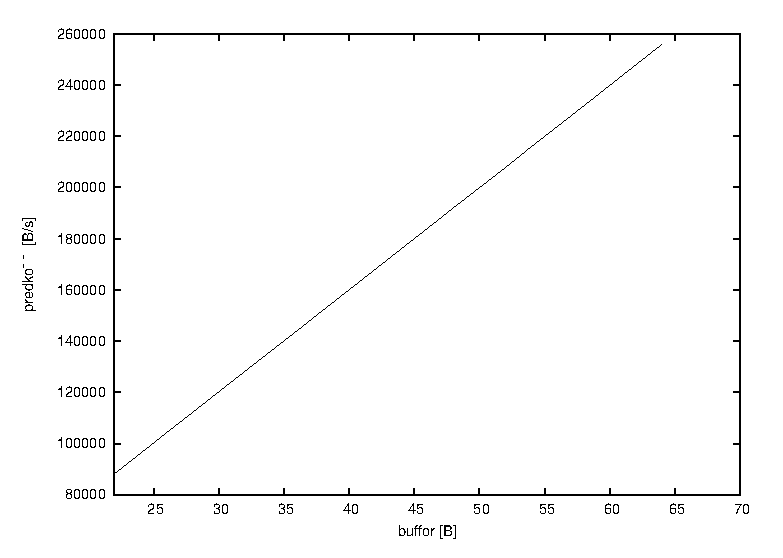
\includegraphics[width=0.75\textwidth]{./img/S_107374200Send}
\caption{Wykres ilustrujący prędkość wysyłania danych w zależności od buffora dla ~102 MB (tryb synchroniczny)}
\label{fig:S_107374200Send}
%\end{figure}
}
\end{figure}
%%todo
Na Rys. \ref{fig:S_107374200Send} widoczny jest wyraźny wzrost szybkości wysyłania danych wraz ze zwiększeniem bufora. Jest to doświadczenie wykonane na stosunkowo małym buforze spowodowane ograniczeniami płytki LandTiger. Wykres jest liniowy 
\begin{figure}[h]
{
\centering
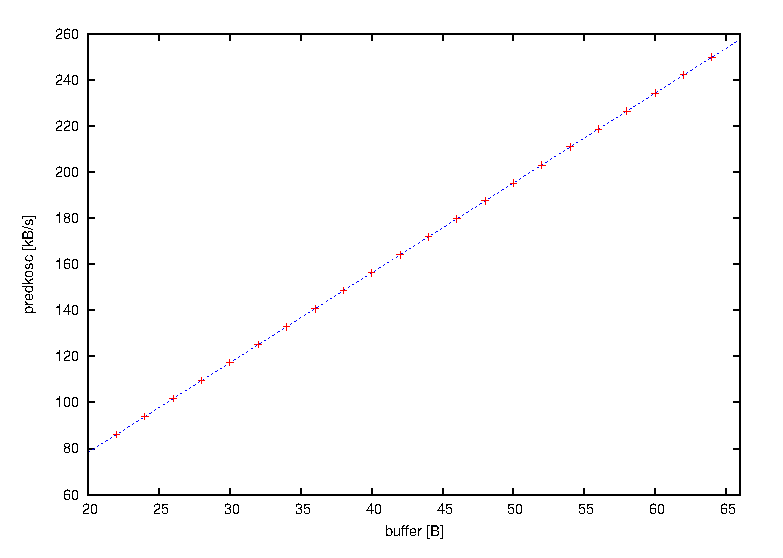
\includegraphics[width=0.7\textwidth]{./img/S_107374200Receive}
\caption{Wykres ilustrujący prędkość odbierania danych w zależności od buffora dla ~102 MB (tryb synchroniczny)}
\label{fig:S_107374200Receive}
%\end{figure}
}
\end{figure}
\newline
Analogiczny wykres widoczny jest dla prędkości odbierania danych (Rys. \ref{fig:S_107374200Receive}), różnice są niezauważalne przy tak małej ilości danych.
%44\begin{figure}[htpb]

%\begin{figure}[H]
%{
%\centering
%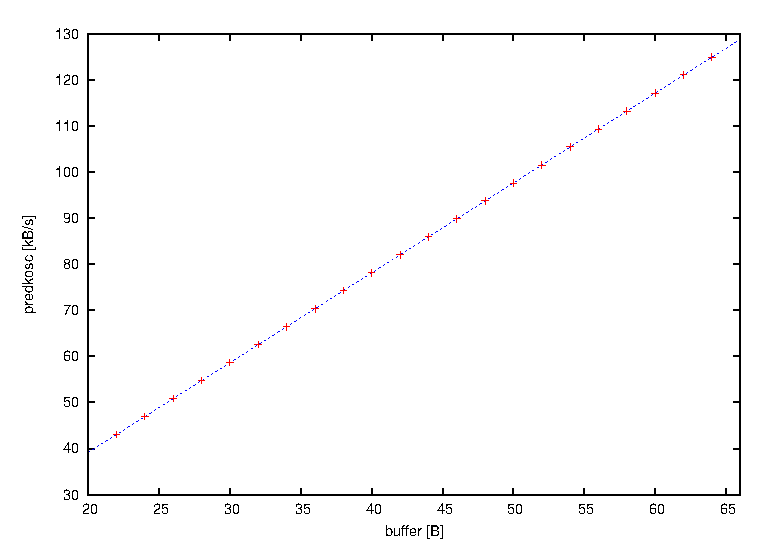
\includegraphics[width=0.75\textwidth]{./img/S_107374200SendReceive}
%\caption{TODO S\_107374200SendReceive.jpg}
%\label{fig:S_107374200SendReceive}
%\end{figure}
%}
%\end{figure}
%%%%%%
\begin{figure}[H]
{
\centering
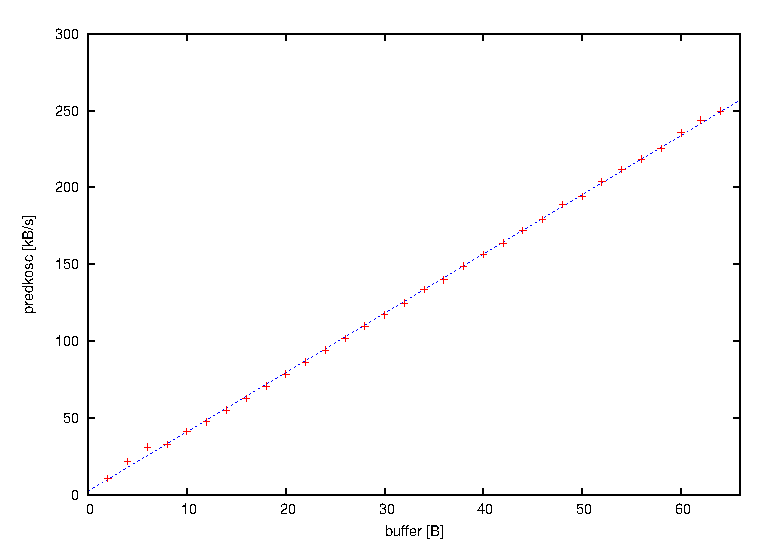
\includegraphics[width=0.7\textwidth]{./img/S_10737420Send}
\caption{Wykres ilustrujący prędkość wysłania danych w zależności od buffora dla ~10 MB (tryb synchroniczny)}
%\end{figure}
\label{fig:S_10737420Send}
}
\end{figure}

W wypadku wysyłania nieco mniejszej próbki danych prędkość obrazuje się jako nieco mniej stabilna. Całość widoczna jest na Rys. \ref{fig:S_10737420Send}. Wykres nie jest już liniowy a prędkość zdaje się być na bardziej niedeterministyczna.

\begin{figure}[H]
{
\centering
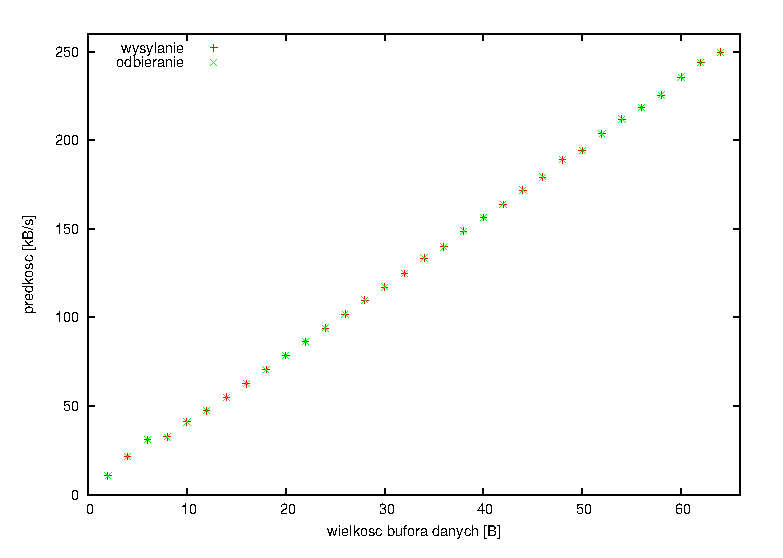
\includegraphics{./img/S_10737420Receive}
\caption{Wykres ilustrujący prędkość odbierania danych w zależności od buffora dla ~10 MB (tryb synchroniczny)}
\label{fig:S_10737420Receive}
%\end{figure}
}
\end{figure}
Podobnie jak w poprzednim przypadku (dla większej ilości danych), wykres prędkości odbierania danych pokrywa się z wykresem prędkości wysyłania danych (Rys. \ref{fig:S_10737420Receive}).

%\begin{figure}[H]
%{
%\centering
%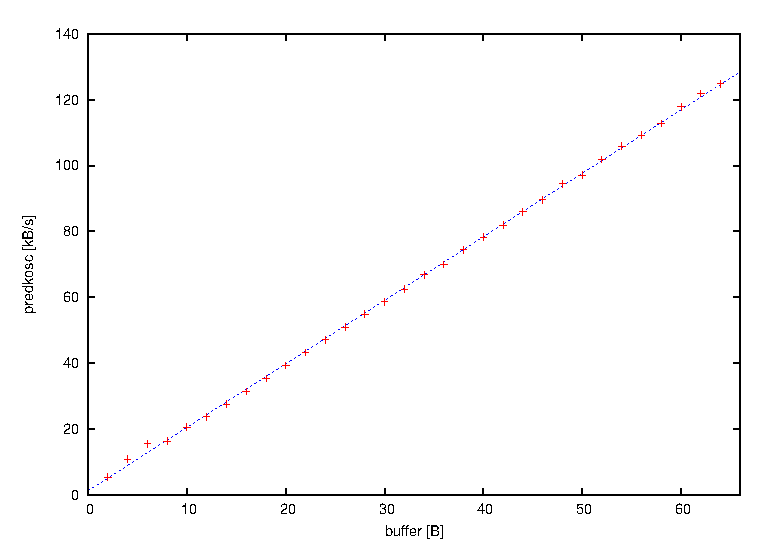
\includegraphics[width=0.75\textwidth]{./img/S_10737420SendReceive}
%\caption{TODO S\_10737420SendReceive.jpg}
%}
%\end{figure}
Podsumowując synchroniczne wysyłanie danych nie należy do najbardziej efektywnych metod. Każda operacja zwraca status i ten status musi być weryfikowany aby zlokalizować ewentualny błąd.
%%%%% Asynch
\newline

Zupełnie innym podejściem charakteryzuje się metoda Asynchroniczna w której korzysta się z nie blokujących metod. Tutaj inną przeszkodą jest to aby to programista zadbał o synchronizacje (ponieważ po łączu w jednym czasie mogą przebiegać dane tylko w jedną stronę). Dzięki tej metodzie istnieje możliwość uzyskania lepszych (szybszych) wyników.
\begin{figure}[H]
{
\centering
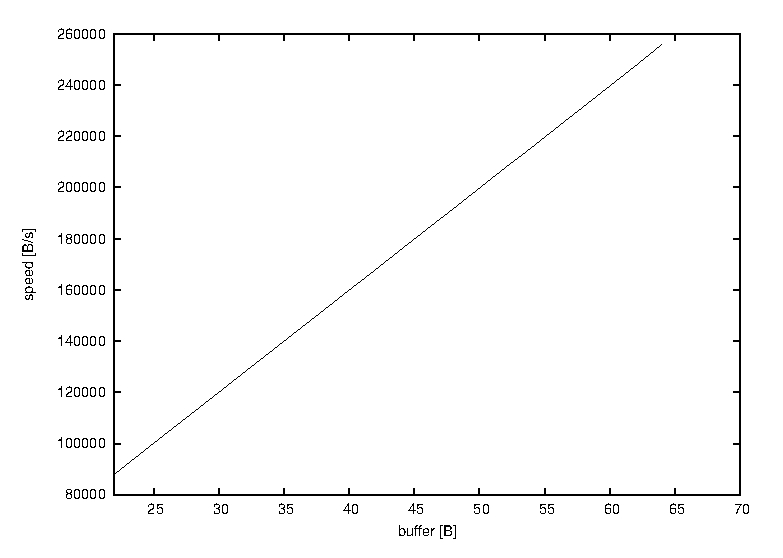
\includegraphics[width=0.72\textwidth]{./img/A_107374200Send}
\caption{Wykres ilustrujący prędkość wysyłania danych w zależności od buffora dla ~102 MB (tryb Asynchroniczny)}
\label{fig:A_107374200Send}
}

\end{figure}

Jak widac na Rys. \ref{fig:A_107374200Send} zależność liniowa również występuje dla tej ilości danych orzy przesyle asynchronicznym, podobnie jak w przypadku przesyłu synchronicznego (Rys. \ref{fig:S_107374200Send}).


\begin{figure}[H]
{
\centering
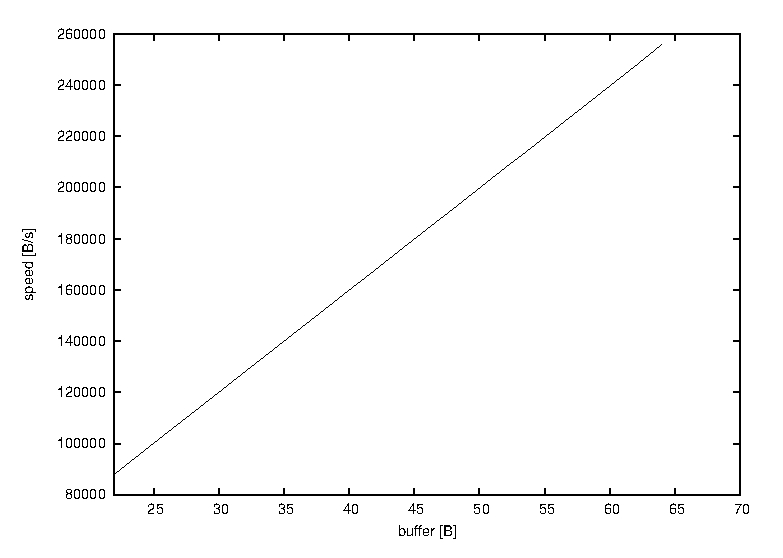
\includegraphics[width=0.72\textwidth]{./img/A_107374200Receive}
\caption{Wykres ilustrujący prędkość odbierania danych w zależności od buffora dla ~102 MB (tryb Asynchroniczny}
\label{fig:A_107374200Receive}
}
\end{figure}
Analogiczna sytuacja występuje w wypadku odbierania danych (o wielkości ~102 MB) metodą asynchroniczną. Wykres jest liniowy jak jego odpowiednik z metody synchronicznej (Rys. \ref{fig:S_107374200Receive}) a wyniki są bardzo zbliżone do siebie.



%%%%%%

\begin{figure}[H]
{
\centering
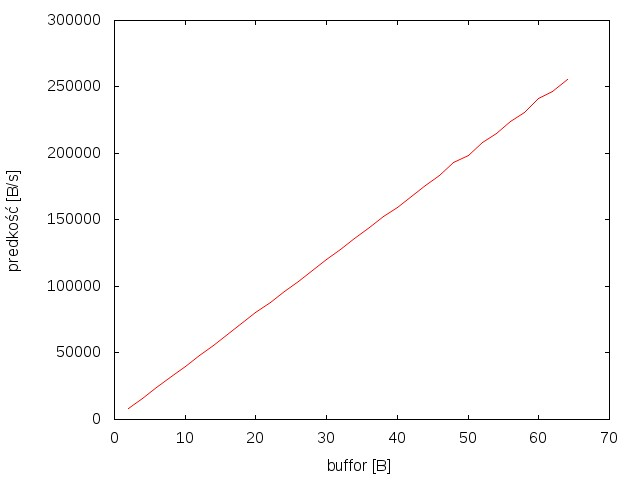
\includegraphics[width=0.75\textwidth]{./img/A_10737420Send}
\caption{Wykres ilustrujący prędkość wysyłania danych w zależności od buffora dla ~10 MB (tryb asynchroniczny)}
\label{fig:A_10737420Send}
}
\end{figure}

Jeśli przeprowadzimy testy dla mniejszej ilości danych to zauważalny jest brak liniowości takiego wykresu (zarówno dla Rys. \ref{fig:A_10737420Send} jak i Rys. \ref{fig:A_10737420Receive}).
\begin{figure}[H]
{
\centering
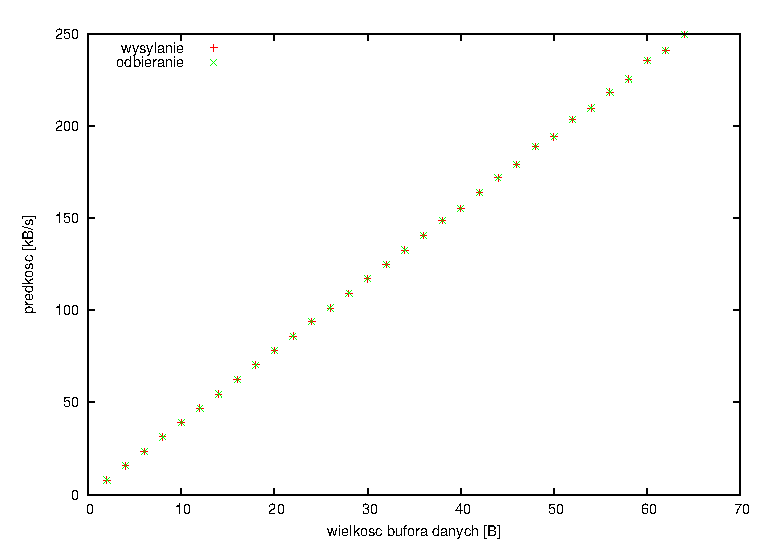
\includegraphics[width=0.75\textwidth]{./img/A_10737420Receive}
\caption{Wykres ilustrujący prędkość odbierania danych w zależności od buffora dla ~10 MB (tryb asynchroniczny)}
\label{fig:A_10737420Receive}
}
\end{figure}

Podsumowując użycie bufora dopuszczalnego przez mikrokontroler LandTiger (czyli bufora nie większego niż 64B) nie jest nawet zbliżona do prędkości porządanej (140 MB/s) bez względu czy korzystaliśmy z synchronicznej metody czy asynchronicznej. Przyczyną jest tutaj wielkość używanego bufora, z powodów dla których LandTiger nie dopuszcza użycia wiekszego bufora niż 64B  pozostałem testy oparte są na zasymulowanych danych. 
\newline

Dodatkowo została przeprowadzona symulacja z uwzględnieniem większego bufora danych ale została wykonana bez poprawnego odbioru danych po stronie kontrolera. Oznacza to że te dane mogą zostać potraktowane jedynie jako przypuszczenia jak wyglądałby wykres gdyby dane były przetworzone prawidłowo. Poniższe (Rys. \ref{fig:S_bbuf1} oraz Rys. \ref{fig:S_bbuf2} wykresy przedstawiają wygenerowane wyniki.

\begin{figure}[H]
{
\centering
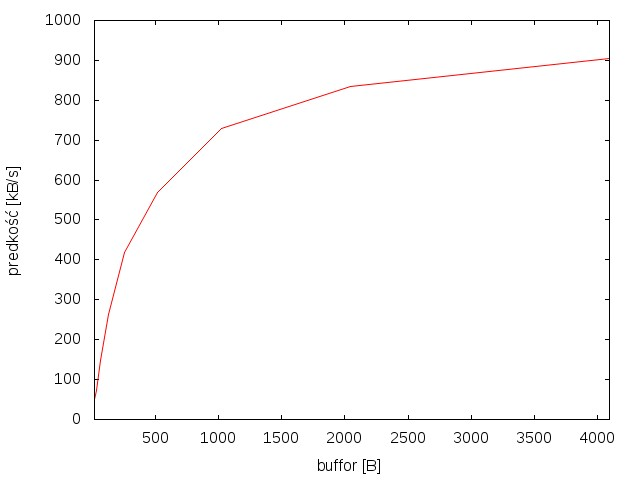
\includegraphics[width=1\textwidth]{./img/S_bbuf1}
\caption{Wykres ilustrujący zmianę prędkości przesyłania danych z użyciem bufora z przedziału 16 B - 4 kB}
\label{fig:S_bbuf1}
}
\end{figure}

Powyższy wykres obrazuje zmianę prędkości wysyłania przy założeniu poprawnego odbioru danych po stronie kontrolera. Zależność liniowa całkowicie zaniknęła. Wartości rozmiaru bufora danych jest podwajana z każdym zgięciem krzywej (początkowa wartość 16 B, końcowa 4096 B = 4 kB), a więc rozbieżność przesyłu danych jest duża. Warto zauważyć iż pomimo dość dużego bufora danych prędkość nie przekroczyła 1 MB/s (max wartość 905,702 kB/s).
\begin{figure}[H]
{
\centering
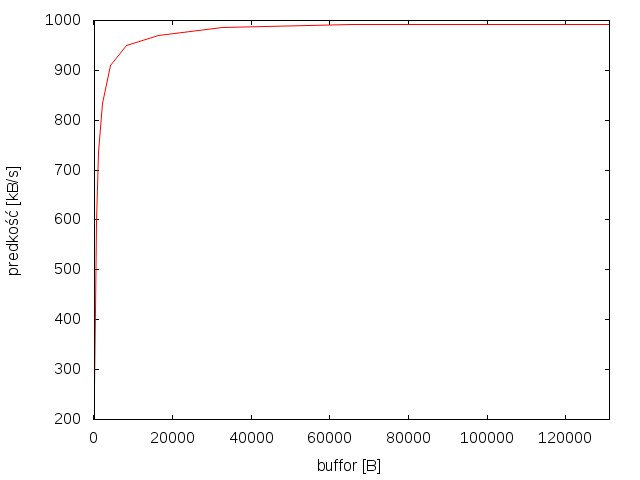
\includegraphics[width=1\textwidth]{./img/S_bbuf2}
\caption{todo:S\_bbuf2}
\label{fig:S_bbuf2}
}
\end{figure}

Powyższy wykres jest rozwinięciem poprzednika. Obrazuje zmianę prędkości na podstawie zasymulowanych danych oraz przy założeniach poprawnego odebrania danych przez mikrokontroler. Podstawową różnicą jest wielkość użytego bufora w tym przypadku. Dla tego przypadku został użyty bufor o wartości minimalnej równe 128 B oraz maksymalnej równej 131072 B (128 kB). Bufor w każdym kroku jest podwajany. Początkowo wartość uzyskiwanej prędkości wzrasta gwałtownie w każdym kroku, natomiast powyżej wartości 8 kB nie są już tak gwałtowne a wręcz krzywa przechodzi w coraz bardziej poziomą i dąży do wartości 1 MB/s. 
\newline

Pomimo zasymulowania dość sporych danych wraz z użyciem dość dużego bufora danych nie udało się uzyskać oczekiwanej minimalnej prędkości. Jednym z powodów jest to, że obsługa odbioru danych została zasymulowana po stronie mikrokontrolera dla bufora danych większego niż 64 B (ograniczenia kontrolera).


\chapter{Podsumowanie}
\label{ConclusionChapter}
Celem projektu było uzyskanie jak największej prędkości przesyłu danych po interfejsie USB. Na wstępie zamieszczone zostało krótkie wprowadzenie odnośnie dostępnych standardów USB oraz ich zarysowi historycznemu. Kolejnym krokiem był dwóch najbardziej popularnych bibliotek do obsługi interfejsu USB (libUSB oraz winUSB). W rozdziale został zawarty krótki opis najważniejszych aspektów bibliotek wraz z uzasadnieniem wyboru libUSB jako tej używanej w projekcie.

Dosyć ważną część odgrywa opis API biblioteki libUsb. Znajduje się w nim dość obszerny opis poszczególnych funkcji użytych w projekcie. Jest to kluczowe aby zrozumieć późniejszą implementację.

W kolejnym rozdziale został przedstawiony mikrokontroler użyty w projekcie, wraz z dokładnym opisem dostępnych funkcjonalności (nie tylko tych użytych w projekcie). Jak okazuję się w kolejnych rozdziałach brakuje mu kluczowej funkcjonalności z punktu widzenia projektu a mianowicie obsługi standardu USB2.0. \cite{landtigerDesc}

Jednym z najważniejszych rozdziałów jest rozdział opisujący sposób implementacji projektu wraz z załączonym kodem źródłowym. Przedstawiony został tam sposób łatwego wywoływania testu oraz opis krok po kroku co zostaje wykonane przed uzyskaniem rezultatu. Zostaje też przedstawiony łatwy sposób rozszerzalności o kolejne klasy implementujące nowy rodzaj testu.
\newline

Rozdział obrazujący rezultaty testów jest najważniejszym w projekcie. Wnioski z wyników nie należą do pozytywnych. Z powodu ograniczeń na mikrokontrolerze w tym ograniczenie obsługi na chipie do standardu USB1.1 (pomimo wlutowanego złącza USB2.0) nie udało się uzyskać minimalnej wymaganej w projekcie prędkości przesyłania danych (17,5 MB/s). Nawet pomimo zasymulowania większego bufora danych (bez poprawnej obsługi odbioru danych po stronie mikrokontrolera w którym zaniechano weryfikacji odebranych danych z powodu niemożności obsługi tak dużego buforu danych).

Warto zaznaczyć, że nie oznacza to iż uzyskanie docelowej prędkości z wykorzystaniem standardu USB2.0 jest nie możliwe (oczywiście z wykorzystaniem innego mikrokontrolera). Standard USB2.0 dopuszcza wielkość bufora 1024 B a co za tym idzie porównując to do obecnej wielkości uzyskamy 16 razy większą.

Na podstawie otrzymanych wyników uzyskanych z wykorzystaniem standardu USB1.1 możemy założyć iż prędkość przesyłu danych z wykorzystaniem USB2.0 oscylowała by w granicach 16 MB/s. Wartość ta jest zależna od odpowiedniej konfiguracji więc możemy dodatkowo przyjąć prędkość 17,5 MB/s jest jak najbardziej osiągalna.


\begin{thebibliography}{1}

\bibitem{embeddedC} Michael J. Pont {\em Embedded C       },  UK: Pearson Education Limited, 2002.

\bibitem{embeddedSystems} Steven F. Barret and Daniel J. Pack {\em Embedded Systems} USA: Pearson Education, Inc., 2005.

\bibitem{USBSystemArch} Don Anderson {\em Universal Serial Bus System Architecture } USA: MindShare, Inc., 1997.

\bibitem{bootstrapLinUSB} Rajaram Regupathy {\em Bootstrap Yourself with Linux-USB Stack: Design, Develop, Debug, and Validate Embedded USB } Course Technology, 2012.

\bibitem{DevUSBPher} Wooi Ming Tan {\em Developing USB PC Peripherals } Annabooks, 1999.

\bibitem{USB20Doc} USB Implementers Forum, Inc., USB2.0 specification reference [online] 
\newline 
\url{http://www.usb.org/developers/docs/usb20_docs/}

\bibitem{USB30Doc} USB Implementers Forum, Inc., USB3.0 and USB2.0 specyfication reference [online] 
\newline 
\url{http://www.usb.org/developers/docs/}

\bibitem{libusbDoc} libusb 2012-2015, libusb documentation reference [online]
\newline 
\url{http://libusb.sourceforge.net/api-1.0/}

\bibitem{libusbDesc} libusb 2012-2015, libusb description reference [online]
\newline 
\url{http://libusb.info/}


\bibitem{winusbDesc} Microsoft 2015, winusb description reference [online]
\newline 
\url{https://msdn.microsoft.com/en-us/library/windows/hardware/ff540196(v=vs.85).aspx}

\bibitem{micrDevAppUSBDev} Microsoft 2015, {\em Developing Windows applications for USB devices} [online]
\newline 
\url{https://msdn.microsoft.com/en-us/library/windows/hardware/dn303342(v=vs.85).aspx}

\bibitem{micrAccUsbDev} Microsoft 2015, {\em How to Access a USB Device by Using WinUSB Functions} [online]
\newline 
\url{https://msdn.microsoft.com/en-us/library/windows/hardware/ff540174(v=vs.85).aspx}

\bibitem{micCommWithUsb} Microsoft 2010, {\em How to Use WinUSB to Communicate with a USB Device} [doc from Microsoft web]
\newline 
\url{http://download.microsoft.com/download/9/C/5/9C5B2167-8017-4BAE-9FDE D599BAC8184A/WinUsb_HowTo.docx}

\bibitem{landtigerDesc} mbed, LandTiger description reference [online]
\newline 
\url{https://developer.mbed.org/users/wim/notebook/landtiger-baseboard/}


\end{thebibliography}

\end{document}